% Options for packages loaded elsewhere
\PassOptionsToPackage{unicode}{hyperref}
\PassOptionsToPackage{hyphens}{url}
\PassOptionsToPackage{dvipsnames,svgnames,x11names}{xcolor}
%
\documentclass[
  sn-mathphys-num,
]{sn-jnl}



\usepackage{amsmath,amssymb}
\usepackage{iftex}
\ifPDFTeX
  \usepackage[T1]{fontenc}
  \usepackage[utf8]{inputenc}
  \usepackage{textcomp} % provide euro and other symbols
\else % if luatex or xetex
  \usepackage{unicode-math}
  \defaultfontfeatures{Scale=MatchLowercase}
  \defaultfontfeatures[\rmfamily]{Ligatures=TeX,Scale=1}
\fi
\usepackage{lmodern}
\ifPDFTeX\else  
    % xetex/luatex font selection
\fi
% Use upquote if available, for straight quotes in verbatim environments
\IfFileExists{upquote.sty}{\usepackage{upquote}}{}
\IfFileExists{microtype.sty}{% use microtype if available
  \usepackage[]{microtype}
  \UseMicrotypeSet[protrusion]{basicmath} % disable protrusion for tt fonts
}{}
\makeatletter
\@ifundefined{KOMAClassName}{% if non-KOMA class
  \IfFileExists{parskip.sty}{%
    \usepackage{parskip}
  }{% else
    \setlength{\parindent}{0pt}
    \setlength{\parskip}{6pt plus 2pt minus 1pt}}
}{% if KOMA class
  \KOMAoptions{parskip=half}}
\makeatother
\usepackage{xcolor}
\setlength{\emergencystretch}{3em} % prevent overfull lines
\setcounter{secnumdepth}{-\maxdimen} % remove section numbering
% Make \paragraph and \subparagraph free-standing
\makeatletter
\ifx\paragraph\undefined\else
  \let\oldparagraph\paragraph
  \renewcommand{\paragraph}{
    \@ifstar
      \xxxParagraphStar
      \xxxParagraphNoStar
  }
  \newcommand{\xxxParagraphStar}[1]{\oldparagraph*{#1}\mbox{}}
  \newcommand{\xxxParagraphNoStar}[1]{\oldparagraph{#1}\mbox{}}
\fi
\ifx\subparagraph\undefined\else
  \let\oldsubparagraph\subparagraph
  \renewcommand{\subparagraph}{
    \@ifstar
      \xxxSubParagraphStar
      \xxxSubParagraphNoStar
  }
  \newcommand{\xxxSubParagraphStar}[1]{\oldsubparagraph*{#1}\mbox{}}
  \newcommand{\xxxSubParagraphNoStar}[1]{\oldsubparagraph{#1}\mbox{}}
\fi
\makeatother


\providecommand{\tightlist}{%
  \setlength{\itemsep}{0pt}\setlength{\parskip}{0pt}}\usepackage{longtable,booktabs,array}
\usepackage{calc} % for calculating minipage widths
% Correct order of tables after \paragraph or \subparagraph
\usepackage{etoolbox}
\makeatletter
\patchcmd\longtable{\par}{\if@noskipsec\mbox{}\fi\par}{}{}
\makeatother
% Allow footnotes in longtable head/foot
\IfFileExists{footnotehyper.sty}{\usepackage{footnotehyper}}{\usepackage{footnote}}
\makesavenoteenv{longtable}
\usepackage{graphicx}
\makeatletter
\def\maxwidth{\ifdim\Gin@nat@width>\linewidth\linewidth\else\Gin@nat@width\fi}
\def\maxheight{\ifdim\Gin@nat@height>\textheight\textheight\else\Gin@nat@height\fi}
\makeatother
% Scale images if necessary, so that they will not overflow the page
% margins by default, and it is still possible to overwrite the defaults
% using explicit options in \includegraphics[width, height, ...]{}
\setkeys{Gin}{width=\maxwidth,height=\maxheight,keepaspectratio}
% Set default figure placement to htbp
\makeatletter
\def\fps@figure{htbp}
\makeatother

%%%% Standard Packages

\usepackage{graphicx}%
\usepackage{multirow}%
\usepackage{amsmath,amssymb,amsfonts}%
\usepackage{amsthm}%
\usepackage{mathrsfs}%
\usepackage[title]{appendix}%
\usepackage{xcolor}%
\usepackage{textcomp}%
\usepackage{manyfoot}%
\usepackage{booktabs}%
\usepackage{algorithm}%
\usepackage{algorithmicx}%
\usepackage{algpseudocode}%
\usepackage{listings}%

%%%%

\raggedbottom
\usepackage{multirow}
\usepackage{centernot}
\makeatletter
\@ifpackageloaded{caption}{}{\usepackage{caption}}
\AtBeginDocument{%
\ifdefined\contentsname
  \renewcommand*\contentsname{Table of contents}
\else
  \newcommand\contentsname{Table of contents}
\fi
\ifdefined\listfigurename
  \renewcommand*\listfigurename{List of Figures}
\else
  \newcommand\listfigurename{List of Figures}
\fi
\ifdefined\listtablename
  \renewcommand*\listtablename{List of Tables}
\else
  \newcommand\listtablename{List of Tables}
\fi
\ifdefined\figurename
  \renewcommand*\figurename{Figure}
\else
  \newcommand\figurename{Figure}
\fi
\ifdefined\tablename
  \renewcommand*\tablename{Table}
\else
  \newcommand\tablename{Table}
\fi
}
\@ifpackageloaded{float}{}{\usepackage{float}}
\floatstyle{ruled}
\@ifundefined{c@chapter}{\newfloat{codelisting}{h}{lop}}{\newfloat{codelisting}{h}{lop}[chapter]}
\floatname{codelisting}{Listing}
\newcommand*\listoflistings{\listof{codelisting}{List of Listings}}
\makeatother
\makeatletter
\makeatother
\makeatletter
\@ifpackageloaded{caption}{}{\usepackage{caption}}
\@ifpackageloaded{subcaption}{}{\usepackage{subcaption}}
\makeatother

\ifLuaTeX
  \usepackage{selnolig}  % disable illegal ligatures
\fi
\usepackage{bookmark}

\IfFileExists{xurl.sty}{\usepackage{xurl}}{} % add URL line breaks if available
\urlstyle{same} % disable monospaced font for URLs
\hypersetup{
  pdftitle={Probabilistic Model of Bilateral Lymphatic Spread in Head and Neck Cancer},
  colorlinks=true,
  linkcolor={blue},
  filecolor={Maroon},
  citecolor={Blue},
  urlcolor={Blue},
  pdfcreator={LaTeX via pandoc}}


\title[Probabilistic Model of Bilateral Lymphatic Spread in Head and
Neck Cancer]{Probabilistic Model of Bilateral Lymphatic Spread in Head
and Neck Cancer}

% author setup
\author*[1,2]{\fnm{Roman} \sur{Ludwig}}\email{roman.ludwig@usz.ch}\author[1,2]{\fnm{Yoel Perez} \sur{Haas}}\email{yoel.perezhaas@usz.ch}\author[1,2]{\fnm{Jan} \sur{Unkelbach}}\email{jan.unkelbach@usz.ch}
% affil setup
\affil[1]{\orgdiv{Department of Physics}, \orgname{University of
Zurich}}
\affil[2]{\orgdiv{Radiation Oncology}, \orgname{University Hospital
Zurich}}

% abstract 

\abstract{Purpose: According to current guidelines for elective nodal
irradiation of oropharyngeal squamous cell carcinoma (OPSCC) patients,
large parts of the contralateral lymphatic system are included in the
elective clinical target volume (CTV-N), even for lateralized tumors
without clinical lymph node involvement in the contralateral neck. In
this work, we present a probabilistic model for bilateral lymphatic
tumor progression in OPSCC to predict the personal risk for occult
disease in any lymph node level (LNL), given the patient's clinical
lymph node involvement, T-stage, and lateralization of the primary
tumor.

Methods: We extend a hidden markov model for lymphatic tumor
progression, which was previously developed for ipsilateral lymph node
involvement, to the contralateral neck. The model represents each of the
LNLs I, II, III, IV, V, and VII of both sides of the neck as a hidden
binary random variable with states healthy and involved. LNLs are
connected to the tumor and among each other via arcs that correspond to
spread probabilities. These spread probability rates are learned via
Markov chain Monte Carlo (MCMC) sampling from a dataset of 833 OPSCC
patients.

Results: The model is able to describe the data on lymph node
involvement well with a small number of interpretable parameters.
Midline extension of the primary tumor is the main risk factor for
contralateral involvement. In addition, the risk of occult metastases in
contralateral lymph node level increases with more advanced T-stage and
more severe ipsilateral involvement. The probability of involvement in
contralateral level III is very low if the upstream level II is
clinically negative. Similarly, the probability of involvement in
contralateral level IV is very low if the upstream level III is
clinically negative.

Conclusions: The model may guide personalized volume reduction of the
elective CTV-N. It suggests that the contralateral neck may be spared
from elective irradiation for lateralized tumors not crossing the
midline. In patients with primary tumors crossing the midline but
clinically negative contralateral neck, the contralateral elective
irradiation may be limited to level II.}

% keywords

\begin{document}
\maketitle


\textsubscript{Source:
\href{https://rmnldwg.github.io/bilateral-paper/manuscript-preview.html}{Article
Notebook}}

\textsubscript{Source:
\href{https://rmnldwg.github.io/bilateral-paper/manuscript-preview.html}{Article
Notebook}}

\section{Introduction}\label{introduction}

When treating head and neck squamous cell carcinomas (HNSCC) with
radiotherapy or surgery, not only the primary tumor and the clinically
detected lymph node metastases are targeted. Per current guidelines,
large volumes of the neck are part of the the elective clinical target
volume (CTV-N)
\citep{gregoire_ct-based_2003, gregoire_delineation_2014, gregoire_delineation_2018, eisbruch_intensity-modulated_2002, biau_selection_2019, chao_determination_2002, vorwerk_guidelines_2011, ferlito_elective_2009}.
This is to minimize the risk of regional recurrences due to untreated
microscopic disease which cannot be detected by current in-vivo imaging
modalities such as computed tomography (CT), magnetic resonance imaging
(MRI), or positron emission tomography (PET). However, minimizing the
risk of missing occult disease in the lymph drainage region must be
balanced against the toxicity related to unnecessary treatment of
healthy tissue.

The aforementioned guidelines for the definition of the CTV-N are based
on anatomically defined lymph node levels (LNL)
\citep{gregoire_delineation_2014} and the overall prevalence of lymph
node metastases in the LNLs. Based on this, they recommend extensive
irradiation of both sides of the neck for a majority of patients.
However, this prevalence the guidelines are based on does not take into
account an individual patient's state of tumor progression, which may
have a great impact on a patient's personal risk for occult disease in a
given LNL. For example, a patient with substantial nodal involvement in
the ipsilateral side and an advanced primary tumor that crosses the
mid-sagittal plane would receive extensive elective irradiation of the
contralateral LNLs II, III, and IVa. However, if the patient presented
with no clinically detectable nodal disease (cN0) and only a small,
clearly lateralized T1 tumor, the same contralateral CTV-N would be
recommended \citep{biau_selection_2019}.

To better quantify this personalized risk of occult disease we have
previously developed an intuitive, probabilistic hidden Markov model
\citep{ludwig_hidden_2021, ludwig_modelling_2023} which was originally
based on a conceptually similar Bayesian network model
\citep{pouymayou_bayesian_2019}. So far, these models were limited to
the ipsilateral side of the neck. The main contribution of this work
will be to extend the formalism to include risk predictions for the
contralateral side as well. We believe this holds the potential to
reduce the electively irradiated volumes in the contralateral neck for
patients whose individual risk for occult disease is low. In turn, this
may substantially reduce the toxicity from irradiation and the
associated decrease in quality of life.

The main contributions of this paper are as follows:

\begin{enumerate}
\def\labelenumi{\arabic{enumi}.}
\item
  In section section~\ref{sec-data} we present a multi-centric dataset
  on lymph node involvement in 833 OPSCC patients. Based on the dataset
  the main risk factors for contralateral lymph node involvement are
  identified and the requirements for the bilateral model extension are
  described (section~\ref{sec-requirements}).
\item
  In section~\ref{sec-ext-to-contra} we present a bilateral HMM of
  lymphatic progression that accounts for the T-stage lateralization of
  the primary tumor as well as clinical involvement as risk factors for
  occult contralateral involvement. In section~\ref{sec-methods} we
  describe how the model training and the computational experiments were
  set up.
\item
  In the results in section~\ref{sec-results}, we demonstrate that the
  model is able to describe the patterns of contralateral lymph node
  involvement observed in the dataset, and we apply the model to
  estimating risk of occult disease for typical patients. In
  section~\ref{sec-discussion}, implications for volume-deescalated
  radiotherapy are discussed.
\end{enumerate}

\section{Data on Lymphatic Progression Patterns}\label{sec-data}

To be able to create models for lymphatic tumor progression that include
all relevant LNLs including the contralateral side, we have collected a
detailed dataset of 833 patients with newly diagnosed oropharyngeal
squamous cell carcinomas
\citep{ludwig_dataset_2022, ludwig_multi-centric_2023}. It reports the
lymph node involvement per LNL of every patient individually in tabular
form, in addition to other primary tumor and patient characteristics
such as T-category, subside, and lateralization of the primary tumor,
and HPV p16 status. Their patient records have been collected at four
different institutions and a brief overview over some of their patients'
characteristics are shown in table~\ref{tbl-data-overview}. The data
from the Inselspital Bern and the Centre Léon Bérard only consist of
patients who received a neck dissection. Since this treatment is more
commonly chosen for early T-category patients, they also make up a
larger portion of the respective dataset. The majority of patients from
the University Hospital Zürich and the Vall d'Hebron Barcelona Hospital
was treated with definitive radiotherapy. For a subset of 83 patients in
the CLB dataset, the lateralization of the primary tumor was not
reported.

\textsubscript{Source:
\href{https://rmnldwg.github.io/bilateral-paper/manuscript-preview.html}{Article
Notebook}}

\begin{longtable}[]{@{}lllllll@{}}

\caption{\label{tbl-data-overview}Overview over the five datasets from
four different institutions used to train and evaluate our model. Here,
we briefly characterize the total number of OPSCC patients from the
respective institution, their median age, what proportion received some
form of neck dissection, the N0 portion of patients, what percentage
presented with early T-category, and the prevalence of primary tumor
midline extension. For a much more detailed look at the data, visit
\href{https://lyprox.org}{lyprox.org}.}

\tabularnewline

\caption{}\label{T_b5301}\tabularnewline
\toprule\noalign{}
Institution & Total & Age (median) & Neck Dissection & N0 & Early T-Cat.
& Mid. Ext. \\
\midrule\noalign{}
\endfirsthead
\toprule\noalign{}
Institution & Total & Age (median) & Neck Dissection & N0 & Early T-Cat.
& Mid. Ext. \\
\midrule\noalign{}
\endhead
\bottomrule\noalign{}
\endlastfoot
Centre Léon Bérard & 325 & 60 & 100\% & 19\% & 69\% & 18\% \\
Inselspital Bern & 74 & 61 & 100\% & 18\% & 66\% & 14\% \\
University Hospital Zurich & 287 & 66 & 26\% & 18\% & 52\% & 31\% \\
Vall d\textquotesingle Hebron Barcelona Hospital & 147 & 58 & 5\% & 21\%
& 34\% & 34\% \\

\end{longtable}

\textsubscript{Source:
\href{https://rmnldwg.github.io/bilateral-paper/manuscript-preview.html}{Article
Notebook}}

\subsection{Consensus on Involvement Status}\label{sec-data-consensus}

Pathological involvement is thus available only for a subset of the
patients and only for the dissected levels. For the remaining patients,
only clinical involvement is available. For the analysis performed in
this paper, all available diagnostic information has been combined into
a consensus decision representing the most likely state of involvement
for each patient and LNL, using literature values for sensitivity and
specificity of different modalities
\citep{de_bondt_detection_2007, kyzas_18f-fluorodeoxyglucose_2008}.
These values are tabulated in table~\ref{tbl-spec-sens}.

This consensus was formed as follows: Suppose the involvement status
\(X_v\) of LNL \(v\) was assessed using different diagnostic modalities
\(\mathcal{O} = \{ \text{MRI}, \text{CT}, \text{pathology}, \ldots \}\),
each characterized by their own pair of sensitivity and specificity
values \(s_N^{\mathcal{o}}\) and \(s_P^{\mathcal{o}}\), with
\(\mathcal{o} \in \mathcal{O}\). Then we have \(|\mathcal{O}|\)
observations \(z_v^{\mathcal{o}} \in \left[ 0, 1 \right]\), where 0
stands for ``healthy'' and 1 for ``involved''. We can then compute the
most likely true involvement \(X_v\) using the likelihood function

\[
\begin{aligned}
\ell \left( X_v \mid \{ z_v^{\mathcal{o}} \}_{\mathcal{o} \in \mathcal{O}} \right) = \prod_{\mathcal{o} \in \mathcal{O}}
\left( 1 - X_v \right) \cdot &\left[ z_v^{\mathcal{o}} \cdot \left( 1 - s_P^{\mathcal{o}} \right) + \left( 1 - z_v^{\mathcal{o}} \right) \cdot s_P^{\mathcal{o}} \right] \\
+ X_v \cdot &\left[ z_v^{\mathcal{o}} \cdot s_N^{\mathcal{o}} + \left( 1 - z_v^{\mathcal{o}} \right) \cdot (1 - s_N^{\mathcal{o}}) \right]
\end{aligned}
\]

We now assume the true state \(X_v\) to take on the value 1 if
\(\ell \left( X_v = 1 \mid \ldots \right) > \ell \left( X_v = 0 \mid \ldots \right)\)
and 0 otherwise. For example, if we have \(z_\text{II}^\text{CT} = 0\)
and \(z_\text{II}^\text{MRI} = 1\) we would compute the following
likelihoods:

\[
\begin{aligned}
\ell \left( X_\text{II} = 1 \mid z_\text{II}^\text{CT} = 0, z_\text{II}^\text{MRI} = 1 \right) &= \left( 1 - s_N^\text{CT} \right) \cdot s_N^\text{MRI} = 15.39\% \\
\ell \left( X_\text{II} = 0 \mid z_\text{II}^\text{CT} = 0, z_\text{II}^\text{MRI} = 1 \right) &= s_P^\text{CT} \cdot \left(1 - s_N^\text{MRI}\right) = 14.44\%
\end{aligned}
\]

In this example, we would thus assume the true state to be involved
(\(X_\text{II} = 1\)).

This method of computing a consensus also ensures that the pathology
reports always override any conflicting clinical diagnosis, due to
pathology's high sensitivity and specificity.

\begin{longtable}[]{@{}lrr@{}}
\caption{Specificity and sensitivity values from the literature
\citep{de_bondt_detection_2007, kyzas_18f-fluorodeoxyglucose_2008}.}\label{tbl-spec-sens}\tabularnewline
\toprule\noalign{}
Modality & Specificity & Sensitivity \\
\midrule\noalign{}
\endfirsthead
\toprule\noalign{}
Modality & Specificity & Sensitivity \\
\midrule\noalign{}
\endhead
\bottomrule\noalign{}
\endlastfoot
CT & 76\% & 81\% \\
PET & 86\% & 79\% \\
MRI & 63\% & 81\% \\
FNA & 98\% & 80\% \\
pathology & 100\% & 100\% \\
\end{longtable}

\subsection{Data Availability}\label{data-availability}

The entire data, including additional patients with tumors in other
primary locations than the oropharynx, is publicly available: It may be
\href{https://lyprox.org/patients/dataset}{downloaded from LyProX} where
it can be interactively explored too,
\href{https://github.com/rmnldwg/lydata}{from GitHub},
\href{https://zenodo.org/search?q=lydata}{from zenodo}, or via the
\emph{Data-in-Brief} publications \citet{ludwig_dataset_2022} and
\citet{ludwig_multi-centric_2023}. The Data-in-Brief publications
contain a detailed description of the datasets and the data format.
However, these publications do not include the most recent dataset
addition from Vall d'Hebron Barcelona Hospital.

\subsection{Patterns of Contralateral Involvement}\label{sec-data-strat}

These datasets allow us to investigate correlations between the
involvement of individual LNLs, or between risk factors and involvement.
In figure~\ref{fig-data-strat}, we have plotted the prevalence of each
contralateral LNL's involvement, stratified by T-category, number of
ipsilaterally involved LNLs, and whether the tumor extended over the
mid-sagittal line. A similar but more complete stratification is also
tabulated in the appendix in table~\ref{tbl-data-strat}.

\begin{figure}

\centering{

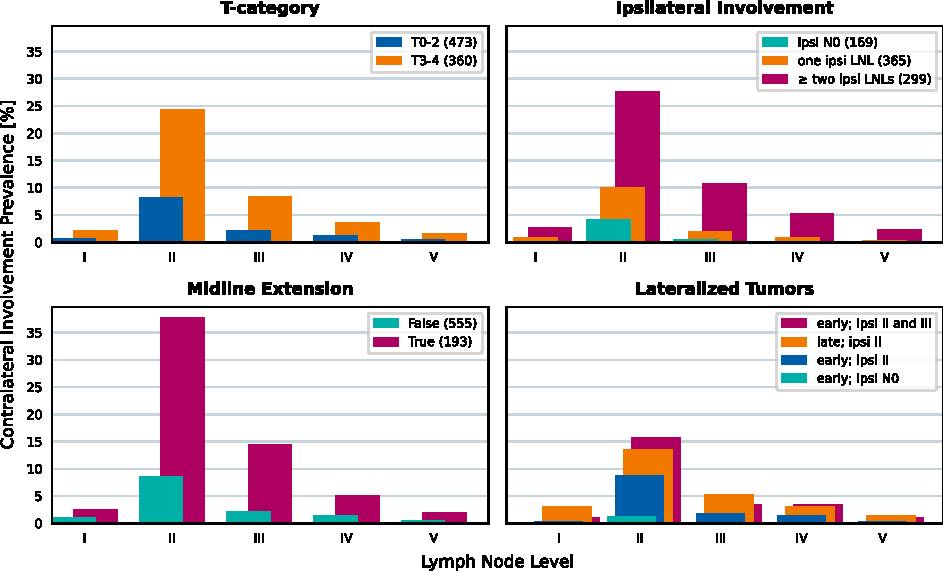
\includegraphics{manuscript_files/mediabag/figures/fig_data_strat.pdf}

}

\caption{\label{fig-data-strat}Contralateral involvement stratified by
T-category (left panel), the number of metastatic LNLs ipsilaterally
(center panel), and whether the primary tumor extended over the
mid-sagittal line or was clearly lateralized (right panel).}

\end{figure}%

The left panel in figure~\ref{fig-data-strat} indicates that T-category
is correlated with contralateral involvement (as it is with overal
involvement). This is simply because T-category may on average be
considered a surrogate for the time between onset of disease and
diagnosis. I.e., a patient with a T4 tumor was -- on average --
diagnosed later than a patient with a T1 tumor. Thus, the former did
have more time to develop metastases.

Similarly, ipsilateral involvement correlates with contralateral
metastasis. The tumor of a patients with many metastases in ipsilateral
LNLs was probably able to spread for longer (or faster) compared to a
tumor in a patient with no nodal disease. This, too, may therefore be
considered a surrogate for the duration of the disease. In addition, it
has been hypothesized that bulky nodal disease ipsilaterally may also
redirect lymph fluids to the contralateral side.

Lastly, the right panel in figure~\ref{fig-data-strat} shows that
patients with a tumor crossing the mid-sagittal line show contralateral
involvement vastly more often compared to patients with clearly
lateralized tumors. This makes intuitive sense, because the lymphatic
system in the head and neck region is typically symmetric and thus no
major vessels cross the midline. Therefore, interstitial fluids from the
primary tumor -- which we assume to carry living malignant cells -- may
only reach the blind-ended lymphatic vessels in the contralateral neck
via short-ranged diffusion. Which in turn is only possible when the
primary tumor is close enough to the mid-sagittal line or crosses it.

The three risk factors for contralateral involvement, midline extension,
T-category, and ipsilateral involvement are correlated. For example,
midline extension was present in 48\% of advanced T-category tumors but
only in 7\% of early T-category tumors. The higher prevalence of
contralateral metastases in advanced T-category tumors may thus be
partially explained by a higher rate of midline extension in these
tumors. However, figure~\ref{fig-data-strat-uncorr} indicates that
advanced T-category and severe ipsilateral involvement do represent
additional risk factors. The figure considers only patients with
lateralized tumors not extending over the midline. For early T-category
and healthy ipsilateral levels I-V, only 1\% (1 out of 84 patients)
shows involvement of contralateral level II. This increases to 5\% (9
out of 165 patients) if ipsilateral level II is involved, to 15\% (9 out
of 60 patients) if ipsilateral levels II and III are involved, and to
23\% (6 out of 26 patients) for advanced T-category with ipsilateral
levels II and III involved.

\begin{figure}

\centering{

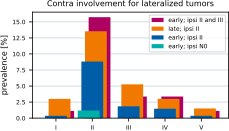
\includegraphics{manuscript_files/mediabag/figures/fig_data_strat_uncorr.pdf}

}

\caption{\label{fig-data-strat-uncorr}Contralateral involvement
prevalence by LNL for lateralized tumors. Shown are four different
scenarios: 1) early T-category with an ipsilateral N0 neck (green), 2)
early T-category with ipsilaterally LNL II involved (blue), 3) late
T-category with ipsilateral LNL II metastatic (orange), and 4) early
T-category with ipsilateral both levels II and III involved (red). This
illustrates that even when controlling for the tumor's lateralization,
T-category and ipsilaeral involvement are predictive of contralateral
metastases.}

\end{figure}%

\subsection{Requirements for a Bilateral Model}\label{sec-requirements}

Based on the observations of the \hyperref[sec-data-strat]{previous
section}, any model to predict the risk for contralateral nodal
involvement, should be able to describe the following:

\begin{enumerate}
\def\labelenumi{\arabic{enumi}.}
\tightlist
\item
  More advanced T-category should lead to higher risk for nodal disease.
  One approach to achieve this via the expected time of diagnosis has
  already been developed in the form of a hidden Markov model
  \citep{ludwig_hidden_2021}.
\item
  The degree of ipsilateral involvement should give the model
  information on the time that may have passed between onset and
  diagnosis of the disease. This should come in addition to what can be
  inferred about the time from T-category alone.
\item
  A tumor that extends over the mid-sagittal line should yield
  contralateral metastases with much higher probability.
\end{enumerate}

Over the course of this work, we will first briefly recap the HMM in
section~\ref{sec-unilateral}, which was so far used to model ipsilateral
lymphatic progression only. Then, we intuitively extend it to include
the contralateral side as well in section~\ref{sec-ext-to-contra}. In
this section, we also introduce a way of modelling the tumor's midline
extension as a random variable (section~\ref{sec-midline}) and lastly
talk about how it may affect the contralateral spread in
section~\ref{sec-params-symmetry}.

\section{Unilateral Model for Lymphatic
Progression}\label{sec-unilateral}

This paper builds on the previously developed unilateral model for
ipsilateral lymph node involvement presented in {[}cite 2024 graph
extension paper{]}. In this section we provide a brief recap of the
unilateral model to introduce the notation needed to extend the
framework to a bilateral model describing both ipsilateral and
contralateral lymph node involvement in section~\ref{sec-ext-to-contra}.
For further details in the ipsilateral model, the reader is referred to
the earlier publications \citep[cite 2024 graph extension
paper]{ludwig_hidden_2021}

We model a patient's state of involvement at an abstract time-step \(t\)
as a vector of hidden binary random variables:

\begin{equation}\phantomsection\label{eq-state-def}{
\mathbf{X}[t] = \begin{pmatrix} X_v[t] \end{pmatrix} \qquad v \in \left\{ 1, 2, \ldots, V \right\}
}\end{equation}

Here, \(V\) is the number of LNLs the model considers. The values a
LNL's hidden binary random variables may take on are \(X_v[t] = 0\)
(\texttt{False}), meaning the LNL \(v\) is healthy or free of metastatic
disease, or \(X_v[t] = 1\) (\texttt{True}), corresponding to some form
of tumor presence (i.e., occult or clinically detected). Since the state
vector \(\mathbf{X}[t]\) is \(V\)-dimensional and binary, there are
\(2^V\) distinct possible lymphatic involvement patterns, which we
enumerate from
\(\boldsymbol{\xi}_0 = \begin{pmatrix} 0 & 0 & \cdots & 0 \end{pmatrix}\)
to
\(\boldsymbol{\xi}_{2^V} = \begin{pmatrix} 1 & 1 & \cdots & 1 \end{pmatrix}\).
In addition, each LNL is associated with an observed binary random
variable \(Z_v\) that describes the clinical involvement of a LNL based
on imaging: \(Z_v = 0\) (\texttt{False}) indicates that the LNL \(v\) is
healthy based on clinical diagnosis, and \(Z_v = 1\) (\texttt{True})
indicates that suspicious lymph nodes were detected that are deemed
metastatic.

Any hidden Markov model is fully described by three quantities:

\begin{enumerate}
\def\labelenumi{\arabic{enumi}.}
\tightlist
\item
  A starting state \(\mathbf{X}[t=0]\) at time \(t=0\) just before the
  patient's tumor formed. In our case, this is always the state where
  all LNLs are still healthy \(\boldsymbol{\xi}_0\).
\item
  The \emph{transition matrix}
  \begin{equation}\phantomsection\label{eq-trans-matrix}{
  \mathbf{A} = \left( A_{ij} \right) = \big( P \left( \mathbf{X}[t+1] = \boldsymbol{\xi}_j \mid \mathbf{X}[t] = \boldsymbol{\xi}_i \right) \big)
  }\end{equation} where the value at row \(i\) and column \(j\)
  represents the probability to transition from state
  \(\boldsymbol{\xi}_i\) to \(\boldsymbol{\xi}_j\) during the time-step
  from \(t\) to \(t+1\). Note that we prohibit self-healing, meaning
  that during a transition, no LNL may change their state from
  \(X_v[t]=1\) to \(X_v[t+1]=0\). Consequently, many elements of the
  transition matrix are zero.
\item
  Lastly, the \emph{observation matrix}
  \begin{equation}\phantomsection\label{eq-obs-matrix}{
  \mathbf{B} = \left( B_{ij} \right) = \big( P \left( \mathbf{Z} = \boldsymbol{\zeta}_j \mid \mathbf{X}[t_D] = \boldsymbol{\xi}_i \right) \big)
  }\end{equation} where in row \(i\) and at column \(j\) we find the
  probability to \emph{observe} a lymphatic involvement pattern
  \(\mathbf{Z} = \boldsymbol{\zeta}_j\), given that the true (but
  hidden) state of involvement at the time of diagnosis \(t_D\) is
  \(\mathbf{X}[t_D] = \boldsymbol{\xi}_i\).
\end{enumerate}

The transition matrix \(\mathbf{A}\) is parametrized using a directed
acyclic graph (DAG) as an abstract representation of the underlying
lymphatic network. Directed arcs from the primary tumor to a LNL are
associated with a probability \(b_v\) for direct spread to LNL \(v\)
during one time step. Directed arcs from a LNL \(v\) to a LNL \(r\) are
associated with a probability \(t_{vr}\) for the tumor to progress from
one LNL to the next. In this paper, we build on the DAG shown in
figure~\ref{fig-full-graph} which was obtained by maximizing the model
evidence as described in {[}cite 2024 graph extension paper{]}.

\begin{figure}

\centering{

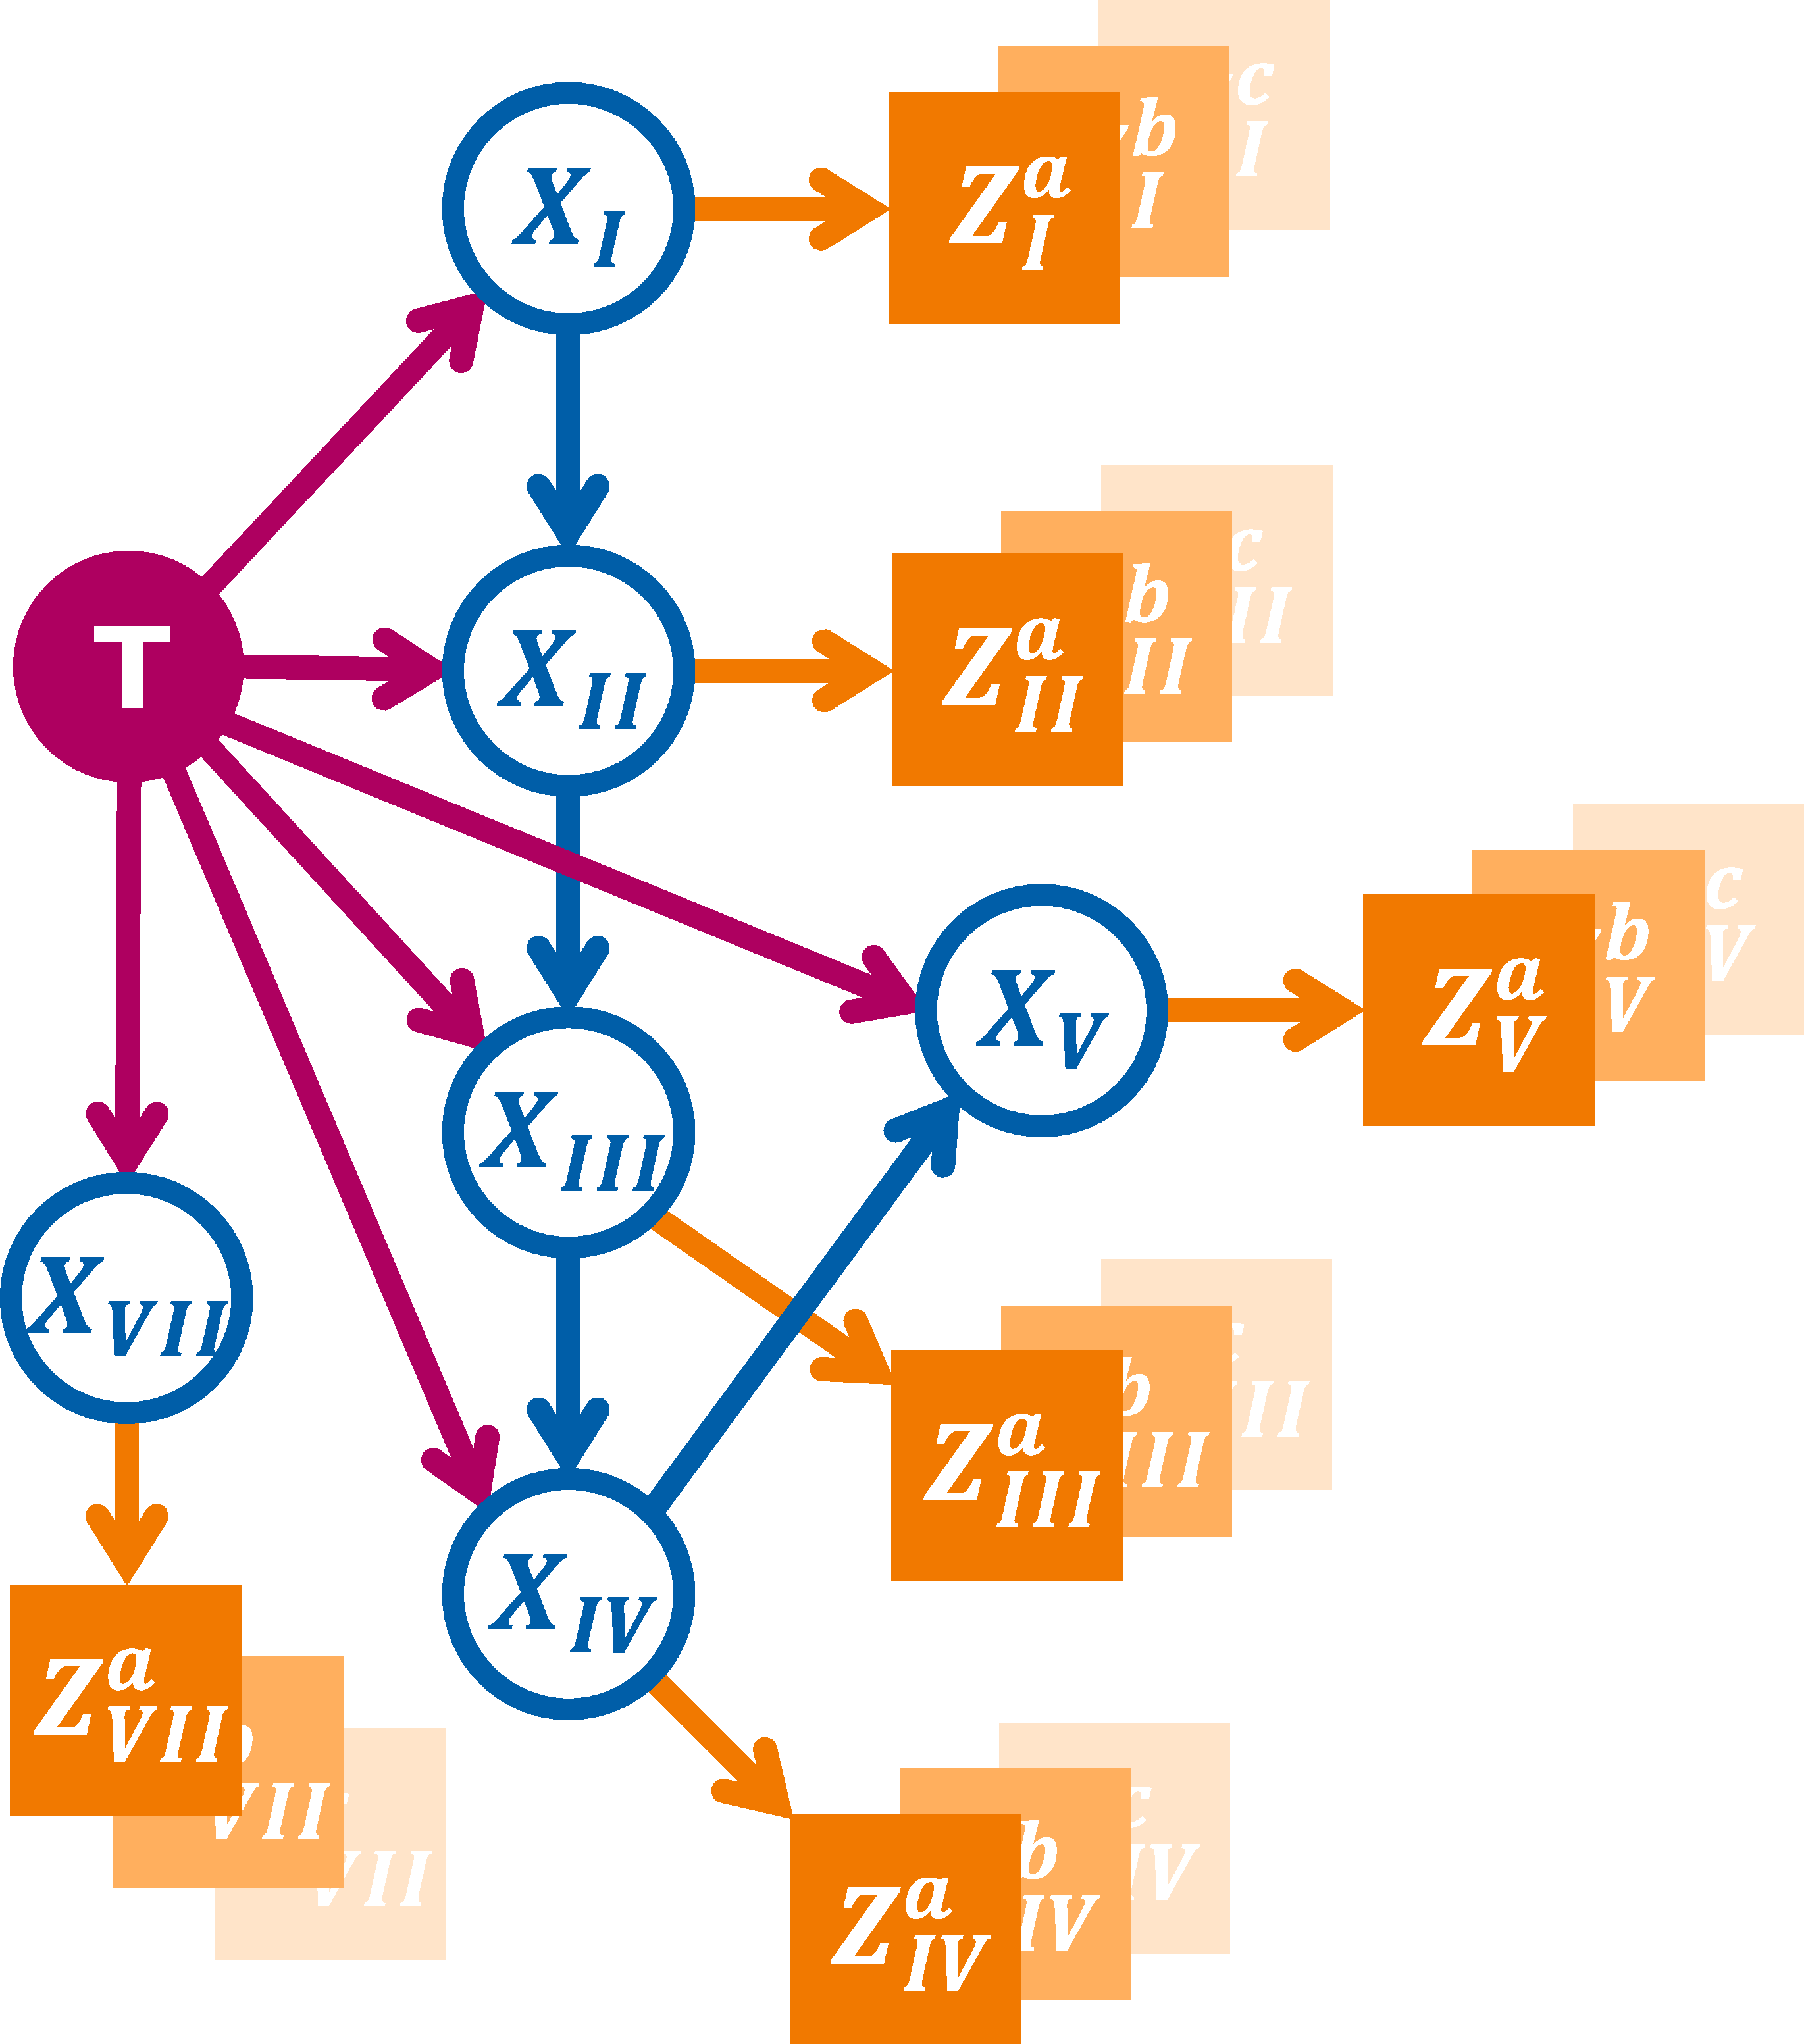
\includegraphics[width=0.4\textwidth,height=\textheight]{manuscript_files/mediabag/static/full-graph.pdf}

}

\caption{\label{fig-full-graph}Directed acyclic graph (DAG) representing
the abstract lymphatic network in the head and neck region. Blue nodes
are the LNLs' hidden random variables, the red node represents the
tumor, and the orange square nodes depict the binary observed variables.
Red and blue arcs symbolize the probability of lymphatic spread along
that edge during one time-step. The orange arcs represent the
sensitivity and specificity of the observational modality (e.g.~CT, MRI,
pathology, \ldots).}

\end{figure}%

Using the introduced quantities, we can evolve the distribution of all
possible hidden states from \(\mathbf{X}[t=0] = \boldsymbol{\xi}_0\)
step by step, by successively multiplying this vector with the
transition matrix \(\mathbf{A}\). For later use, we define at this point
the matrices of the dsitributions over all hidden states, given all
time-steps \(\boldsymbol{\Lambda}\):

\begin{equation}\phantomsection\label{eq-lambda-matrix}{
\boldsymbol{\Lambda} = P \left( \mathbf{X} \mid \mathbf{t} \right) = \begin{pmatrix}
\boldsymbol{\pi}^\intercal \cdot \mathbf{A}^0 \\
\boldsymbol{\pi}^\intercal \cdot \mathbf{A}^1 \\
\vdots \\
\boldsymbol{\pi}^\intercal \cdot \mathbf{A}^{t_\text{max}} \\
\end{pmatrix}
}\end{equation}

Where the \(k\)-th row in this matrix corresponds to the probability
distribution over hidden states after \(t=k-1\) time-steps.

At the time of the diagnosis \(t_D\), we multiply the result with the
observation matrix \(\mathbf{B}\). We may then look up the likelihood of
a patient presenting with the diagnosis
\(\mathbf{Z}=\boldsymbol{\zeta}_i\) in the \(i\)-th entry of the final
result. However, the remaining issue is that the value of \(t_D\) is
unknown, i.e.~over how many time-steps the HMM should be evolved. We
solve this problem by marginalizing over the time of diagnosis.
Different distributions over the diagnosis times can then be choosen
based on T-category. For instance, the mean of the time-prior to
marginalize over the diagnosis time for early T-category patients
\(P\left( t_D \mid \text{early} \right)\) may be shifted towards earlier
times than the one for advanced T-category patients
\(P\left( t_D \mid \text{early} \right)\). This gives us for example

\[
P\left( \mathbf{X} \mid \text{T}x = \text{early} \right) = \sum_{t=0}^{t_\text{max}} P \left( \mathbf{X} \mid t \right) \cdot P(t \mid \text{early})
\]

In this work, we use binomial distributions
\(\mathfrak{B} \left( t_D, p_{\text{T}x} \right)\) as time-priors which
have one free parameter \(p_{\text{T}x}\) for each group of patients we
differentiate based on T-category. Also, we fix \(t_\text{max} = 10\),
which means that the expected number of time-steps from the onset of a
patient's disease to their diagnosis is
\(\mathbb{E}\left[ t_D \right] = 10 \cdot p_{\text{T}x}\).

\subsection{Likelihood Function of the Unilateral
Model}\label{likelihood-function-of-the-unilateral-model}

With the formalism introduced above, we can write the likelihood
function for a patient to present with a diagnosis consisting of an
observed state and a T-category
\(d = \left( \boldsymbol{\zeta}_i, \text{T}x \right)\) as follows:

\begin{equation}\phantomsection\label{eq-single-patient-llh}{
\ell = P \left( \mathbf{Z} = \boldsymbol{\zeta}_i \mid \text{T}x \right) = \sum_{t=0}^{t_\text{max}} \left[ \boldsymbol{\xi}_0 \cdot \mathbf{A}^t \cdot \mathbf{B} \right]_i \cdot P \left( t \mid \text{T}x \right)
}\end{equation}

Above, the quantity inside \(\left[ \ldots \right]_i\) denotes the
\(i\)-th component of the vector that is the result of the vector and
matrix multiplications in the square brackets. Note that it is also
possible to account for missing involvement information: If a diagnosis
(like fine needle aspiration (FNA)) is only available for a subset of
all LNLs, we can sum over all those possible complete observed states
\(\boldsymbol{\zeta}_j\) that match the provided diagnosis.

The single-patient likelihood \(\ell\) in
equation~\ref{eq-single-patient-llh} depends on the spread parameters
shown in figure~\ref{fig-full-graph} via the transition matrix
\(\mathbf{A}\) and on the binomial parameters \(p_{\text{T}x}\) via
time-priors. In this work, we will only differentiate between ``early''
(T1 \& T2) and ``advanced'' (T3 \& T4) T-categories. Therefore, the
parameter space of the unilateral model is:

\begin{equation}\phantomsection\label{eq-param-space}{
\boldsymbol{\theta} = \left( \left\{ b_v \right\}, \left\{ t_{vr} \right\}, p_\text{early}, p_\text{adv.} \right) \quad \text{with} \quad \genfrac{}{}{0pt}{2}{v\leq V}{r\in\operatorname{pa}(v)}
}\end{equation}

And it is our goal to infer the values of these parameters for a given
dataset \(\mathcal{D} = \left( d_1, d_2, \ldots, d_N \right)\) of OPSCC
patients. The likelihood of these \(N\) diagnoses is simply the product
of their individual likelihoods as defined in
equation~\ref{eq-single-patient-llh}. For numerical reasons, we
typically compute the data likelihood in log space:

\begin{equation}\phantomsection\label{eq-log-likelihood}{
\log \mathcal{L} \left( \mathcal{D} \mid \boldsymbol{\theta} \right) = \sum_{i=1}^N \log \ell_i
}\end{equation}

The methodology we use to infer the model's parameters is detailed in
section~\ref{sec-sampling}.

\section{Extension to a Bilateral Model}\label{sec-ext-to-contra}

A naive approach to model the contralateral lymphatic spread would be to
simply employ two independent unilateral models as introduced in
section~\ref{sec-unilateral}. During training, one could enforce that
some parameters are shared between these two models, e.g.~the
parameterization of the distributions over diagnose times or the spread
among the LNLs (\$t\_\{vr\}). However, this approach lacks a way to
describe the correlation between ipsi- and contralateral involvement
discussed in section \{\#sec-data-strat\}. Two independent unilateral
models would not describe the observation that contralateral involvement
becomes more likely with more severe ipsilateral involvement.

Thus, we extend the formalism in section~\ref{sec-unilateral} in such a
way that the model's ipsi- and contralateral side evolve synchronously
over time. To achieve that, we start by writing down the posterior
distribution of involvement an analogy to
equation~\ref{eq-uni-bayes-law}, which is now a joint probability of an
involvement \(\mathbf{X}^\text{i}\) ipsilaterally \emph{and} an
involvement \(\mathbf{X}^\text{c}\) contralaterally, given a diagnosis
of the ipsilateral LNLs \(\mathbf{Z}^\text{i}\) and of the contralateral
ones \(\mathbf{Z}^\text{c}\):

\begin{equation}\phantomsection\label{eq-bilateral-bayes}{
P \left( \mathbf{X}^\text{i}, \mathbf{X}^\text{c} \mid \mathbf{Z}^\text{i}, \mathbf{Z}^\text{c} \right) = \frac{P \left( \mathbf{Z}^\text{i}, \mathbf{Z}^\text{c} \mid \mathbf{X}^\text{i}, \mathbf{X}^\text{c} \right) P \left( \mathbf{X}^\text{i}, \mathbf{X}^\text{c} \right)}{P \left( \mathbf{Z}^\text{i}, \mathbf{Z}^\text{c} \right)}
}\end{equation}

For the sake of brevity, we omit the dependency on the parameters and
the T-category here.

The probability of the diagnoses given a hidden state factorises:
\(P \left( \mathbf{Z}^\text{i}, \mathbf{Z}^\text{c} \mid \mathbf{X}^\text{i}, \mathbf{X}^\text{c} \right) = P \left( \mathbf{Z}^\text{i} \mid \mathbf{X}^\text{i} \right) \cdot P \left( \mathbf{Z}^\text{c} \mid \mathbf{X}^\text{c} \right)\),
and the two factors are described through observation matrices
\(\mathbf{B}^\text{i}\) and \(\mathbf{B}^\text{c}\).

The term representing the model's prior probability of hidden
involvement does not factorize. However, we assume that there is no
direct lymph drainage from an ipsilateral LNL to a contralateral LNL. No
major lymph vessels cross the mid-sagittal plane. In the graphical
model, this means that we assume no directed arcs between ipsilateral
and contralateral LNLs, i.e.~tumor spread to the contralateral side is
due to the primary tumor alone. We can thus write the joint probability
\(P \left( \mathbf{X}^\text{i}, \mathbf{X}^\text{c} \right)\) as a
factorising sum:

\begin{equation}\phantomsection\label{eq-bilateral-marginal}{
\begin{aligned}
P \left( \mathbf{X}^\text{i}, \mathbf{X}^\text{c} \right) &= \sum_{t=0}^{t_\text{max}} P(t) \cdot P \left( \mathbf{X}^\text{i}, \mathbf{X}^\text{c} \mid t \right) \\
&= \sum_{t=0}^{t_\text{max}} P(t) \cdot P \left( \mathbf{X}^\text{i} \mid t \right) \cdot P \left( \mathbf{X}^\text{c} \mid t \right)
\end{aligned}
}\end{equation}

This assumption makes intuitive sense: The state of the ipsilateral and
contralateral sides of the lymphatic network evolves independently over
time as there are no major lymph vessels crossing the midline. However,
both sides are coupled via time. Qualitatively speaking, according to
the model in \{\#eq-bilateral-marginal\}, a joint state with severe
contralateral involvement and limited ipsilateral involvement would be
unlikely, because severe contralateral involvement becomes likely only
at later time steps when limited ipsilateral involvement becomes
unlikely.

Using \{\#eq-bilateral-marginal\} along with
equation~\ref{eq-lambda-matrix}, we can write the above distribution
algebraically as a product:

\begin{equation}\phantomsection\label{eq-bilateral-marginal-algebra}{
P \left( \mathbf{X}^\text{i} = \boldsymbol{\xi}_n, \mathbf{X}^\text{c} = \boldsymbol{\xi}_m \right) = \left[ \boldsymbol{\Lambda}^\intercal_\text{i} \cdot \operatorname{diag} P(\mathbf{t}) \cdot \boldsymbol{\Lambda}_\text{c} \right]_{n,m}
}\end{equation}

\subsection{Parameter Symmetries}\label{sec-params-symmetry}

In general, the matrices \(\boldsymbol{\Lambda}_\text{i}\) and
\(\boldsymbol{\Lambda}_\text{c}\) could be parameterized using a
disjoint set of parameters, i.e., the ipsi- and contralateral spread
rates are entirely different. However, using three sensible assumptions,
we can reduce the parameter space by sharing some parameters between the
two sides:

\begin{enumerate}
\def\labelenumi{\arabic{enumi}.}
\tightlist
\item
  We assume that both ipsilateral and contralateral spread is described
  through the same graph shown in \{\#fig-full-graph\}.
\item
  We assume the spread \emph{among} the LNLs to be same on both sides.
  It is reasonable to assume the lymphatic system is symmetric. Thus,
  the spread rates from one LNL to the other should be symmetric, too.
  Formally, this means\\
  \begin{equation}\phantomsection\label{eq-symmetries}{
  \begin{aligned}
  b_v^\text{c} &\neq b_v^\text{i} \\
  t_{rv}^\text{c} &= t_{rv}^\text{i}
  \end{aligned}
  }\end{equation} for all \(v \leq V\) and
  \(r \in \operatorname{pa}(v)\).
\item
  The tumor's spread to the contralateral side in case of an extension
  over the midline is larger than if it was clearly lateralized, but
  smaller than its spread to the ipsilateral side. This assumption stems
  from a simple thought experiment: Consider moving the tumor from a
  clearly lateralized position accross the mid-sagittal plane to the
  same position, but on the contralateral side. In the beginning we
  would have \(b_v^\text{c} < b_v^\text{i}\), while in the end, the
  situation is reversed. If a tumor extends over the mid-sagittal line,
  its contralateral spread rate can be expected to be in between these
  two extremes. We encode this in a \emph{mixing parameter}
  \(\alpha \in [0,1]\) that captures a ``degree of asymmetry'':\\
  \begin{equation}\phantomsection\label{eq-mixing}{
  b_v^{\text{c},\epsilon=\texttt{True}} = \alpha \cdot b_v^\text{i} + (1 - \alpha) \cdot b_v^{\text{c},\epsilon=\texttt{False}}
  }\end{equation} This means the model now uses three different sets of
  parameters to describe the spread from the tumor to the LNLs:
  \(b^\text{i}_v\) for the spread to the ipsilateral LNLs,
  \(b_v^{\text{c},\epsilon=\texttt{False}}\) for the spread to the
  contralateral LNLs as long as the tumor is clearly lateralized, and
  finally \(b_v^{\text{c},\epsilon=\texttt{True}}\) when it crosses the
  midline. Note, however, that these three sets of spread rates only
  account for \(2 \cdot 2^V + 1\) parameters, since they are coupled via
  the mixing parameter \(\alpha\).
\end{enumerate}

Our parameter space has now expanded to

\begin{equation}\phantomsection\label{eq-bi-param-space}{
\boldsymbol{\theta} = \left( \left\{ b_v^\text{i} \right\}, \left\{ b_v^\text{c} \right\}, \alpha, \left\{ t_{vr} \right\}, p_\text{early}, p_\text{adv.} \right) \quad \text{with} \quad \genfrac{}{}{0pt}{2}{v\leq V}{r\in\operatorname{pa}(v)}
}\end{equation}

which is less than double in size, compared to the unilateral model.
From these parameters, we now build three different transition matrices:
The unchanged matrix \(\mathbf{A}_\text{i}\) for the ipsilateral side,
one \(\mathbf{A}_\text{c}^{\epsilon=\texttt{False}}\) for the
contralateral side that covers the progression as long as the tumor is
lateralized, and \(\mathbf{A}_\text{c}^{\epsilon=\texttt{True}}\) in
case of a tumor that has crossed the mid-sagittal line.

\subsection{Modelling Midline Extension}\label{sec-midline}

It can be assumed that most tumors that cross the midline at the time of
diagnose have started as lateralized tumors and grew over the midline at
a later time step. Hence, the transition matrix
\(\mathbf{A}_\text{c}^{\epsilon=\texttt{True}}\) only applies for a
subset of the time steps. Therefore, we also model the tumor's extension
over the mid-sagittal line as a binary random variable. A tumor starts
lateralized and at every time-step there is a finite probability
\(p_\epsilon\) that the tumor grows over the midsaggital plane. The
overall probabilities to find a patient with a clearly lateralized tumor
or one that extends over the mid-sagittal line after \(t\) time-steps
are then respectively given by

\[
\begin{aligned}
P(\epsilon = \texttt{False} \mid t) &= (1 - p_\epsilon)^t \\
P(\epsilon = \texttt{True} \mid t) &= 1 - P(\epsilon = \texttt{False} \mid t)
\end{aligned}
\]

Using this, it is straightforward to write down the matrix of state
distributions for all time-steps, as in equation~\ref{eq-lambda-matrix}
covering the contralateral hidden state evolution:

\[
\boldsymbol{\Lambda}_\text{c}^{\epsilon=\texttt{False}} =
\left(
\begin{array}{r}
\boldsymbol{\pi}^\intercal \cdot \left( \mathbf{A}_\text{c}^{\epsilon=\texttt{False}} \right)^{0\phantom{t_\text{max}}} \\
(1-p_\epsilon) \cdot \boldsymbol{\pi}^\intercal \cdot \left( \mathbf{A}_\text{c}^{\epsilon=\texttt{False}} \right)^{1\phantom{t_\text{max}}} \\
\hfill \vdots \hfill \\
(1-p_\epsilon)^{t_\text{max}} \cdot \boldsymbol{\pi}^\intercal \cdot \left( \mathbf{A}_\text{c}^{\epsilon=\texttt{False}} \right)^{t_\text{max}\phantom{0}} \\
\end{array}
\right)
\]

where we used the transition matrix
\(\mathbf{A}_\text{c}^{\epsilon=\texttt{False}}\) that depends on the
base spread parameters \(b_v^{\text{c},\epsilon=\texttt{False}}\).

The case when midline extension is eventually present is more
complicated: We already marginalize over the exact time-step when the
tumor grows over the mid-sagittal line. But whenever that happens, we
also need to change the contralateral transition matrix to use the
increased spread rates \(b_v^{\text{c}, \epsilon=\texttt{True}}\) from
the tumor to the contralateral LNLs, given by the linear mixing in
equation~\ref{eq-mixing}. We can achieve the correct marginalization by
iteratively building the joint distribution
\(P \left( \mathbf{X}^\text{c}, \epsilon=\texttt{True} \mid t \right)\).
We start from \(t=0\), where we know that all LNLs are healthy (the
contralateral neck is in the state
\(\mathbf{X}_\text{c}=\boldsymbol{\xi}_0\)) and the tumor is lateralized
(\(\epsilon=\texttt{False}\)):

\[
P \left( \mathbf{X}^\text{c} = \boldsymbol{\xi}_0, \epsilon=\texttt{False} \mid t=0 \right) = 1
\]

whereas all other states have zero probability. Then we consider an
arbitrary later time-step \(t=\tau+1\). There are two possible scenarios
we need to marginalize over:

\begin{enumerate}
\def\labelenumi{\arabic{enumi}.}
\tightlist
\item
  The tumor was still lateralized at \(t=\tau\) and just grew over the
  midline. Under this scenario, the probability for having a midline
  extension at \(t=\tau+1\) is given by \(p_\epsilon\). We use this to
  weight the contralateral state distribution that was so far evolved
  without increased contralateral spread.
\item
  The mid-sagittal line was already crossed by the tumor. In that case,
  the probability is 1 to remain in that lateralization state. Thus, to
  account for this case we simply add the distribution
  \(P\left( \mathbf{X}^\text{c}, \epsilon=\texttt{True} \mid \tau \right)\)
  from one time-step earlier, arriving at a recursion relation:
\end{enumerate}

\[
P \left( \mathbf{X}^\text{c}, \epsilon=\texttt{True} \mid \tau + 1 \right) = \big[ p_\epsilon P \left( \mathbf{X}^\text{c}, \epsilon=\texttt{False} \mid \tau \right) + P \left( \mathbf{X}^\text{c}, \epsilon=\texttt{True} \mid \tau \right) \big]^\top \cdot \mathbf{A}_\text{c}^{\epsilon=\texttt{True}}
\]

We can collect the iteratively computed distributions for the midline
extension case to define the matrix over the states given all
time-steps, in analogy to equation~\ref{eq-lambda-matrix}:

\[
\boldsymbol{\Lambda}_\text{c}^{\epsilon=\texttt{True}} = \begin{pmatrix}
P \left( \mathbf{X}^\text{c}, \epsilon=\texttt{True} \mid 0 \right) \\
P \left( \mathbf{X}^\text{c}, \epsilon=\texttt{True} \mid 1 \right) \\
\vdots \\
P \left( \mathbf{X}^\text{c}, \epsilon=\texttt{True} \mid t_\text{max} \right) \\
\end{pmatrix}
\]

Using this, we can again write the joint of ipsi- and contralateral
involvement - now also for the case of mid-sagittal extension -
algebraically as before in equation~\ref{eq-bilateral-marginal-algebra}:

\[
P \left( \mathbf{X}^\text{i} = \boldsymbol{\xi}_n, \mathbf{X}^\text{c} = \boldsymbol{\xi}_m, \epsilon \right) = \left[ \boldsymbol{\Lambda}^\intercal_\text{i} \cdot \operatorname{diag} P(\mathbf{t}) \cdot \boldsymbol{\Lambda}_\text{c}^\epsilon \right]_{n,m}
\]

We can use this term to compute the likelihood of all patients with and
without midline extension separately. And if for some patients the
information of tumor lateralization is not available, we can simply sum
the above term once for \(\epsilon=\texttt{False}\) and once for
\(\epsilon=\texttt{True}\) to marginalize over the unknown variable.

The final parameter space of our extended model has now reached this
size:

\begin{equation}\phantomsection\label{eq-ext-param-space}{
\boldsymbol{\theta} = \left( \left\{ b_v^\text{i} \right\}, \left\{ b_v^\text{c} \right\}, \alpha, \left\{ t_{vr} \right\}, p_\text{early}, p_\text{adv.}, p_\epsilon \right) \quad \text{with} \quad \genfrac{}{}{0pt}{2}{v\leq V}{r\in\operatorname{pa}(v)}
}\end{equation}

\subsection{Model Prediction in the Bayesian
Context}\label{model-prediction-in-the-bayesian-context}

Our stated goal is to compute the risk for a patient's true ipsi- and
contralateral nodal involvement states \(\mathbf{X}^\text{i}\) and
\(\mathbf{X}^\text{c}\), \emph{given} their individual diagnosis
\(d = \left( \boldsymbol{\zeta}^\text{i}_k, \boldsymbol{\zeta}^\text{c}_\ell, \epsilon, \text{T}x \right)\).
Here, this diagnosis consists of the observed ipsi- and contralateral
nodal involvements, the patient's midline extension \(\epsilon\), and
their tumor's T-category \(\text{T}x\). Using Bayes' law, we can write
this risk as:

\begin{equation}\phantomsection\label{eq-uni-bayes-law}{
P \big( \mathbf{X}^\text{i}, \mathbf{X}^\text{c} \mid d, \boldsymbol{\hat{\theta}} \big)
= \frac{P \left( \boldsymbol{\zeta}^\text{i}_k \mid \mathbf{X}^\text{i} \right) P \left( \boldsymbol{\zeta}^\text{c}_\ell \mid \mathbf{X}^\text{c} \right) P \big( \mathbf{X}^\text{i}, \mathbf{X}^\text{c}, \epsilon \mid \boldsymbol{\hat{\theta}}, \text{T}x \big)}
{\sum_{i=0}^{2^V} \sum_{j=0}^{2^V} P \left( \boldsymbol{\zeta}^\text{i}_k \mid \mathbf{X}^\text{i}=\boldsymbol{\xi}^\text{i}_i \right) P \big( \boldsymbol{\zeta}^\text{c}_\ell \mid \mathbf{X}^\text{c}=\boldsymbol{\xi}^\text{c}_j \big) P \big( \mathbf{X}^\text{i}=\boldsymbol{\xi}^\text{i}_i, \mathbf{X}^\text{c}=\boldsymbol{\xi}^\text{c}_j, \epsilon \mid \boldsymbol{\hat{\theta}}, \text{T}x \big)}
}\end{equation}

The terms
\(P \left( \boldsymbol{\zeta}^\text{i}_k \mid \mathbf{X}^\text{i} \right)\)
and
\(P \left( \boldsymbol{\zeta}^\text{c}_\ell \mid \mathbf{X}^\text{c} \right)\)
are defined solely by sensitivity and specificity of the diagnostic
modality. Terms like these already appeared in the definition of the
observation matrx in equation~\ref{eq-obs-matrix}. The \emph{prior}
\(P \big( \mathbf{X}^\text{i}, \mathbf{X}^\text{c}, \epsilon \mid \boldsymbol{\hat{\theta}}, \text{T}x \big)\)
in the above equation is the crucial term that is supplied by a trained
model and its parameters \(\boldsymbol{\hat{\theta}}\).

It is possible to compute this \emph{posterior} probability of true
involvement not only for one fully defined state
\((\mathbf{X}^\text{i}, \mathbf{X}^\text{c})\), but also for
e.g.~individual LNLs: For example, the risk for involvement in the
contralateral level IV would be a marginalization over all ipsilateral
states \(\boldsymbol{\xi}^\text{i}_i\) and all contralateral states
\(\boldsymbol{\xi}^\text{c}_j\) where \(\xi^\text{c}_{j4}=1\). Formally:

\begin{equation}\phantomsection\label{eq-marg-over-posterior}{
P \big( \text{cIV} \mid \mathbf{Z}^\text{i}=\boldsymbol{\zeta}^\text{i}_k, \mathbf{Z}^\text{c}=\boldsymbol{\zeta}^\text{c}_\ell, \boldsymbol{\hat{\theta}}, \text{T}x \big) = \sum_k \sum_{\ell \, : \, \xi_{\ell 4}=1} P \big( \mathbf{X}^\text{i} = \boldsymbol{\xi}^\text{i}_k, \mathbf{X}^\text{c} = \boldsymbol{\xi}^\text{c}_\ell \mid \boldsymbol{\zeta}^\text{i}_k, \boldsymbol{\zeta}^\text{c}_\ell, \epsilon, \boldsymbol{\hat{\theta}}, \text{T}x \big)
}\end{equation}

\section{Computational methods}\label{sec-methods}

In this section, we detail how the experiments were performed. Every
figure, table, and result is fully reproducible via the GitHub
repository
\href{https://github.com/rmnldwg/bilateral-paper}{\texttt{rmnldwg/bilateral-paper}}.
It also contains the raw manuscript and instructions on how to recreate
all figures, tables, and the final document.

\subsection{Involvement Data
Consensus}\label{involvement-data-consensus}

It is possible to provide our model with multiple different diagnostic
modalities, each being characterized by different pairs of sensitivity
and specificity. However, we instead chose to combine them into a single
``consensus'' diagnosis before parameter inference, as introduced in
\textbf{?@sec-sec-data-consensus}. We opted for this because the
literature values of sensitivity and specificity
\citep{de_bondt_detection_2007, kyzas_18f-fluorodeoxyglucose_2008} of
imaging modalities like MRI and CT do not plausibly match some of our
observations: In the USZ cohort, 78\% of OPSCC patients where diagnosed
with ipsilateral LNL II involvement via diagnostic imaging. This is
virtually impossible with sensitivities around 80\% and specificities
lower than 100\%.

\subsection{MCMC Sampling}\label{sec-sampling}

For parameter inference, we used the Python package
\href{https://emcee.readthedocs.io/en/stable/}{\texttt{emcee}}
\citep{foreman-mackey_emcee_2013}. It implements efficient MCMC sampling
algorithms that employ multiple parallel samplers for affine invariance
and better performance on multi-core CPUs. The sample proposal
algirothms used by us are based on differential evolution moves
\citep{ter_braak_differential_2008, nelson_run_2013}. The
\href{https://emcee.readthedocs.io/en/stable/}{\texttt{emcee}} library
was provided with the likelihood implemented by our
\href{https://lymph-model.readthedocs.io/en/stable/}{\texttt{lymph-model}}
Python package.

For each dimension in the parameter space of the model, we initialized
12 of these parallel samplers, called ``walkers'', with random values in
the unit cube. Every time all of these walkers advanced 50 steps, the
autocorrelation time of the chains was estimated. For short chains, this
estimate is not trustworthy, but stabilizes for longer chains. We
therefore considered a sampling to be converged when two criteria were
met:

\begin{enumerate}
\def\labelenumi{\arabic{enumi}.}
\tightlist
\item
  The change in the autocorrelation time was less then 5.0e-2.
\item
  The estimate of the autocorrelation dropped below \(n\) / 50 where
  \(n\) is the length of the chain up to that point.
\end{enumerate}

All samples up to this convergence - called the \emph{burn-in phase} -
were discarded. We only kept another 10 samples after that, which were
spaced 10 steps apart.

First, in figure~\ref{fig-model-burnin-history}, we verify the sampling
converged successfully by inspecting two monitoring quantities: The
autocorrelation time of the MCMC chain and the acceptance fractions of
the parallel walkers.

\begin{figure}

\centering{

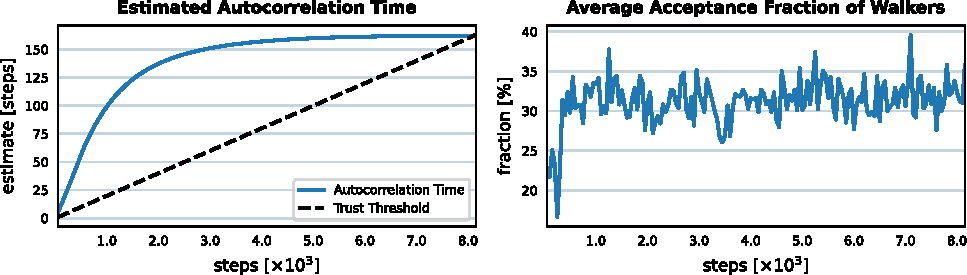
\includegraphics{manuscript_files/mediabag/figures/fig_model_burnin_history.pdf}

}

\caption{\label{fig-model-burnin-history}Monitoring quantities during
the burn-in phase of the parameter sampling. Left: The autocorrelation
time of the sampling chain estimated at different sampling steps. We
consider the chain converged when the estimate of the autocorrelation
time is stable and drops below the trust threshold of \(n/50\) where
\(n\) is the number of steps. Right: Fraction of accepted MCMC proposals
averaged over all parallel walkers. Values around 30\% indicate good
mixing of the walkers.}

\end{figure}%

\subsection{Computing the Observed and Predicted Prevalence of
Involvement Patterns}\label{sec-prevalence}

We want to assess the model's capability to approximate the distribution
of lymphatic involvement patterns seen in the data. To that end, we
compare the prevalence of some invovlement patterns under selected
scenarios with the model's prediction for how often these involvements
it expects to see, given these scenarios.

In this context, a ``scenario'' includes the patient's T-category
\(\text{T}x\) and whether the patient's tumor extended over the
mid-sagittal line, i.e.~\(\epsilon=\texttt{True}\) or
\(\epsilon=\texttt{False}\).

An involvement pattern specifies for each ipsi- and contralateral LNL
whether it is ``healthy'', ``involved'', or ``masked''. If it is
``masked'', we essentially state that we are not interested in the
involvement of that LNL and the prevalence will be marginalized over
this LNL's involvement.

For example, we may be interested in the prevalence of contralateral LNL
II involvement (i.e., contra LNL II ``involved'' and all other LNLs
``masked'') under the scenario of early T-category (T0-T2) and no
midline extension (\(\epsilon=\texttt{False}\)). To compute this
prevalence in the data, we select all patients of this scenario (in our
data, this amounts to 379 patients). Of those, 28 were found to harbor
metastases in their contralateral LNL II. Therefore, the prevalence is
7\%.

When displaying this data prevalence, we often choose to draw a
\emph{beta posterior} over the ``true'' prevalence, hinting at the fact
that our data merely represents a limited sample. The beta posterior
follows from a uniform beta distribution as prior and a binomial
likelihood for the number of patients with the involvement of interest,
given the parameer for the ``true'' prevalence. The resulting
distribution has its maximum at the observed prevalence, but in addition
gives a visual intuition for the variance of of the observed quantity.
I.e., when we observe 3 out of 10 events, the beta posterior is much
wider than if we observe 300 out of 1000 for he same prevalence. It also
allows us to check not only if the model is accurate, but also whether
it reflects the uncertainty contained in the data.

Predicting the prevalence using our model amounts to computing the
following probability:

\[
P \left( \text{II}^\text{c} \mid \epsilon=\texttt{False}, \text{T}x=\text{early} \right) = \frac{P \left( \text{II}^\text{c}, \epsilon=\texttt{False} \mid \text{T}x=\text{early} \right)}{P \left( \epsilon=\texttt{False} \mid \text{T}x=\text{early} \right)}
\]

In the enumator, we marginalize over all ipsi- and contralateral LNLs'
involvements, except for LNL II contralaterally. This is similar to the
marginalization in equation~\ref{eq-marg-over-posterior}, although we
are summing over different quantities. In the denominator, we can simply
insert the joint distribution over midline extension and diagnose time
\(P \left( \epsilon, t \right)\) marginalized over \(t\) using the early
T-category's time-prior.

Since we compare it to the data, which does not report true but only
observed involvement -- although pathologically investigated LNLs may be
as close as possible to the ground truth -- we do not consider
posteriors of the form \(P \left( \mathbf{X} \mid \mathbf{Z} \right)\)
here. Instead, we compute probabilities of observed involvement
\(P \left( \mathbf{Z} \right)\), as in the likelihood
equation~\ref{eq-single-patient-llh}.

When plotted, we usually display histograms over the model's
predictions. Each of their values was computed from a different
parameter set drawn during MCMC sampling, effectively giving us a
distribution over the prevalences. Ideally, the histograms approximate
the location and width of the Beta posteriors when attempting to
describe the data they were trained on.

Note that we decided to omit the y-axis ticks and labels in these
figures over prevalences and risks. The y-axis in these plots measures
the probability density and its numerical values are not intuitively
interpretable. Instead, we occasionally use the freed space to label
e.g.~rows of subplots.

\section{Results: Model evaluation}\label{sec-results}

In table~\ref{tbl-midline-params}, we tabulate the mean and standard
deviation of the sampled parameters for the full midline model.
Considering the parameters of the bilateral model that describe the
ipsilateral spread (\(b^i_v\), \(t_{vr}\) and \(p_\text{adv.}\)), we
note that the bilateral model mostly reproduces the parameter values
reported in the earlier publication \citep{ludwig_modelling_2023} for
the unilateral model. The small differences may be mostly due to the
differences in training dataset. Therefore, the analysis of the models
capability to adequately describe ipsilateral lymph node involvement is
not repeated here and we focus instead on the analysis of contralateral
involvement. We can further note that the contralateral spread
parameters \(b^c_v\) are small compared to the ipsilateral parameters
\(b^i_v\), reflecting the low prevalence of contralateral lymph node
involvement for lateralized tumors.

\textsubscript{Source:
\href{https://rmnldwg.github.io/bilateral-paper/manuscript-preview.html}{Article
Notebook}}

\begin{longtable}[]{@{}lll@{}}

\caption{\label{tbl-midline-params}Mean sampled parameter estimates of
the midline model and the respective standard deviation.}

\tabularnewline

\caption{}\label{T_6f0e6}\tabularnewline
\toprule\noalign{}
Parameter & Mean & Std. Dev. \\
\midrule\noalign{}
\endfirsthead
\toprule\noalign{}
Parameter & Mean & Std. Dev. \\
\midrule\noalign{}
\endhead
\bottomrule\noalign{}
\endlastfoot
Mid. ext. probability & 8.16\% & ± 0.48\% \\
ipsi: T ➜ I & 2.80\% & ± 0.26\% \\
ipsi: T ➜ II & 34.89\% & ± 1.40\% \\
ipsi: T ➜ III & 5.45\% & ± 0.66\% \\
ipsi: T ➜ IV & 0.94\% & ± 0.18\% \\
ipsi: T ➜ V & 1.83\% & ± 0.22\% \\
ipsi: T ➜ VII & 2.32\% & ± 0.26\% \\
contra: T ➜ I & 0.29\% & ± 0.09\% \\
contra: T ➜ II & 2.46\% & ± 0.29\% \\
contra: T ➜ III & 0.14\% & ± 0.07\% \\
contra: T ➜ IV & 0.19\% & ± 0.08\% \\
contra: T ➜ V & 0.05\% & ± 0.04\% \\
contra: T ➜ VII & 0.50\% & ± 0.17\% \\
Mixing ⍺ & 33.87\% & ± 4.32\% \\
I ➜ II & 62.50\% & ± 16.69\% \\
II ➜ III & 14.23\% & ± 1.64\% \\
III ➜ IV & 15.86\% & ± 1.93\% \\
IV ➜ V & 14.58\% & ± 3.76\% \\
late T-cat. binom. prob. & 44.98\% & ± 1.99\% \\

\end{longtable}

\textsubscript{Source:
\href{https://rmnldwg.github.io/bilateral-paper/manuscript-preview.html}{Article
Notebook}}

\subsection{Illustration of the model}\label{illustration-of-the-model}

In this subsection we illustrate parts of the mathematical framework
defined in the previous section. In figure~\ref{fig-model-midext-evo}
(top panel), we visualize the prior distribution over diagnose times
\(P(t)\). By parameter choice, early T-category tumors are diagnosed on
average after 3 time steps. Advanced T-category tumors are diagnosed on
average after 4.5 time steps (\(p_\text{adv.}=0.45\)) , a parameter
learned from the data to describe the higher involvement for advanced
T-category tumors. The probability per time step for the tumor to grow
over the midline, \(p_\epsilon = 0.0816\) yields the probability of
midline extension \(P(\epsilon \mid t)\) at a given time step \(t\) (red
line). The parameter is adjusted such that the model yields the correct
proportion of patients with tumors extending over the midline seen in
the dataset. The bottom panel in figure~\ref{fig-model-midext-evo} shows
the joint probability \(P(\epsilon, t)\) to be diagnosed at time step
\(t\) with a given state of midline extension and T-category.

\begin{figure}

\centering{

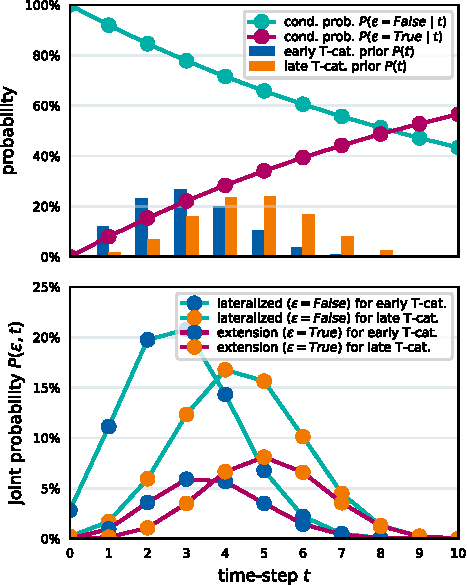
\includegraphics[width=0.5\textwidth,height=\textheight]{manuscript_files/mediabag/figures/fig_model_midext_evo.pdf}

}

\caption{\label{fig-model-midext-evo}The top panel shows the prior
probability to get diagnosed at time-step \(t\) for early and late
T-category tumors as bars. Also in the top panel, we plot the
conditional probability of the tumor's midline extension
(\(\epsilon=\texttt{True}\)), given the time-step \(t\) as a line plot.
In the bottom panel, we show the joint probability of getting diagnosed
in time-step \(t\) \emph{and} having a tumor that crosses the midline.}

\end{figure}%

The model introduced in the previous section defines a model of the
joint probability distribution over midline extension and ipsi- and
contralateral lymph node involvement,
\(P \left( \mathbf{X}^\text{i}, \mathbf{X}^\text{c}, \epsilon \right)\).
How this quantity is computed is illustrated in
figure~\ref{fig-model-state-dist}, visually representing
equation~\ref{eq-bilateral-marginal-algebra}. To keep it manageable to
interpret, this example only considers the LNLs II, III, and IV ipsi-
and contralaterally, resulting in \(2^3 = 16\) distinct states per side
and thus \(2 \times 8 \times 8 = 128\) total states. LNLs I, V, and VII
and the associated spread parameters have been removed from the model
while the remaining parameters are set to the mean values in table xxx.
figure~\ref{fig-model-state-dist} shows the joint distribution as two
separate heatmaps for the two midline extension states for
early/advanced??? T-category tumors. The most likely state is a
lateralized tumor with involvement of ipsilateral level II and no
contralateral involvement, which has a probability of approximately
25\%. The second most probable state is a lateralized tumor with
ipsilateral involvement of levels II and III and no contralateral
involvement. The most likely state with contralateral involvement are
tumors with midline extension with involvement of contralateral level II
and ipsilateral level II and III.

\begin{figure}

\centering{

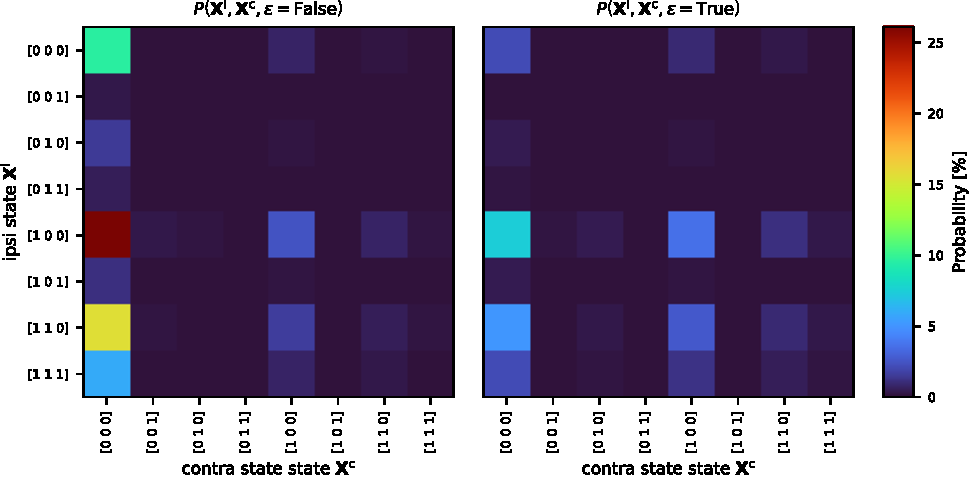
\includegraphics{manuscript_files/mediabag/figures/fig_model_state_dist.pdf}

}

\caption{\label{fig-model-state-dist}Visual representation of
equation~\ref{eq-bilateral-marginal-algebra} for the case of midline
extention. The left and right matrix represent the evolution of the
possible hidden states for the ipsi- and contralateral neck
respectively. In particular, the right matrix describes the evolution of
the contralateral hidden states \emph{and} midline extension. In the
center, the time-prior is plotted as a diagonal matrix. The result of
this matrix computation is the joint distribution
\(P \left( \mathbf{X}^\text{i}, \mathbf{X}^\text{c}, \epsilon=\texttt{True} \right)\)}

\end{figure}%

\subsection{Prevalence predictions for contralateral
involvement}\label{prevalence-predictions-for-contralateral-involvement}

The bilateral model was designed to fulfil the requirements laid out in
section~\ref{sec-requirements}. Now, we investigate to what extent the
model can quantitatively describe the patterns of lymph node involvement
observed in the dataset. To that end, we compare the model's predictions
for contralateral involvement against observations in the data. This is
done given scenarios that differ in T-category and/or midline extension
and/or ipsilateral involvement.

\subsubsection{Dependence of Contralateral Involvement on T-Category and
Midline
Extension}\label{dependence-of-contralateral-involvement-on-t-category-and-midline-extension}

In figure~\ref{fig-model-prevalences-overall}, we plot the prevalence of
contralateral involvement of the LNLs II, III, and IV for the four
scenarios made up of the possible combinations of early and late
T-category, as well as lateralized and midline extending tumors.

\begin{figure}

\centering{

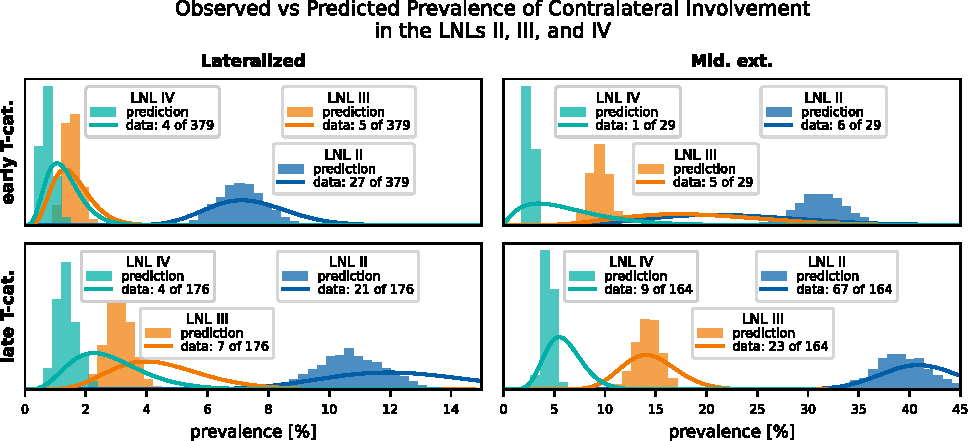
\includegraphics{manuscript_files/mediabag/figures/fig_model_prevalences_overall.pdf}

}

\caption{\label{fig-model-prevalences-overall}Comparison of predicted
(histograms) vs observed (beta posteriors) prevalences. Shown for the
contralateral LNLs II (blue), III (orange), and IV (green). The top row
shows scenarios with early T-category tumors, the bottom row for late
T-category ones. The left column depicts scenarios where the primary
tumor is clearly lateralized, the right column scenarios of tumors
extending over the mid-sagittal line. This figure illustrates the
model's ability to describe the prevalence of involvement for different
combinations of the risk factors T-category and midline extension.}

\end{figure}%

Figure~\ref{fig-model-prevalences-overall} shows nicely that the model
is capable of accurately accounting for the most important risk factors,
i.e.~T-category and midline extension. As observed in the data, the
model predicts that the prevalence of contralateral LNL II involvement
increases from below 8\% for early T-category lateralized tumors to
almost 40\% when the tumor is of advanced T-category and crosses the
mid-sagittal line. Similarly, the prevalence of contralateral LNL III
involvement increases from around 2\% for early T-category lateralized
tumors to almost 15\% when the tumor is of advanced T-category and
crosses the mid-sagittal line.

\subsubsection{Correlation between Ipsi- and Contralateral
Involvement}\label{correlation-between-ipsi--and-contralateral-involvement}

\begin{figure}

\centering{

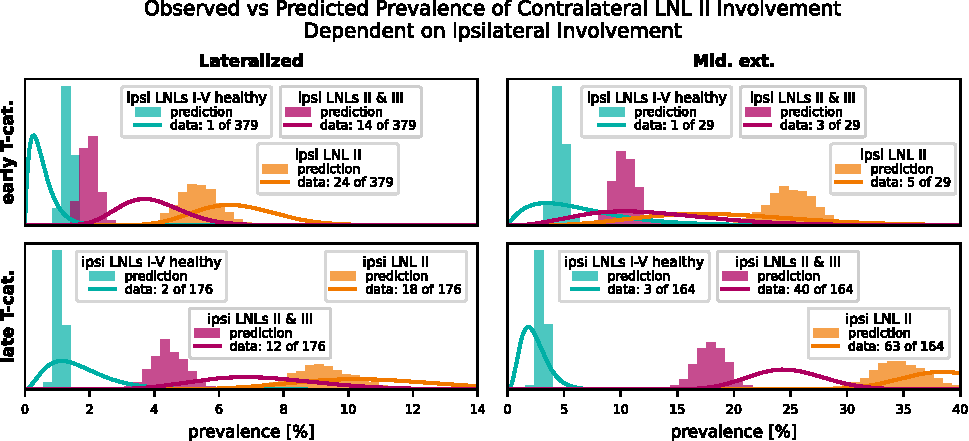
\includegraphics{manuscript_files/mediabag/figures/fig_model_prevalences_with_ipsi.pdf}

}

\caption{\label{fig-model-prevalences-with-ipsi}Comparison of the
computed and observed prevalences for scenarios that illustrate the
model's capability of accounting for the correlation between ipsi- and
contralateral involvement. We show two scenarios: One where the
ipsilateral neck shows no involvement (at least LNLs I to V are healthy,
LNL VII was ignored because data on it is missing for some patients) in
blue and one where at least LNL III was involved in orange. These two
scenarios are plotted for all combinations of T-category (early in top
row, advanced in bottom row) and tumor lateralization (lateralized in
left column, extending over mid-sagittal line in right column).}

\end{figure}%

In figure~\ref{fig-model-prevalences-with-ipsi} we display the model's
ability to capture the correlation between ipsi- and contralateral
involvement. It shows that the prevalence of metastases in the two sides
of the neck is correlated via the time of diagnosis, despite the model
not having any direct connections between the two side. However, there
are some discrepancies in the model's prediction: It cannot quite
capture the correlation of ipsi- and contralateral involvement that is
seen in the data. This is notable for example in the bottom right
subplot where the prevalence is overestimated for the scenario of an
(almost) healthy ipsilateral neck and underestimated when at least LNL
III shows metastases. One reason for this may be the width of the
time-prior: If it was wider, the posterior over the diagnosis time given
the ipsilateral involvement could more flexibly shift to reflect a more
severe contralateral involvement.

\subsubsection{Influence of Upstream Involvement on Contralateral
Metastasis}\label{influence-of-upstream-involvement-on-contralateral-metastasis}

\begin{figure}

\centering{

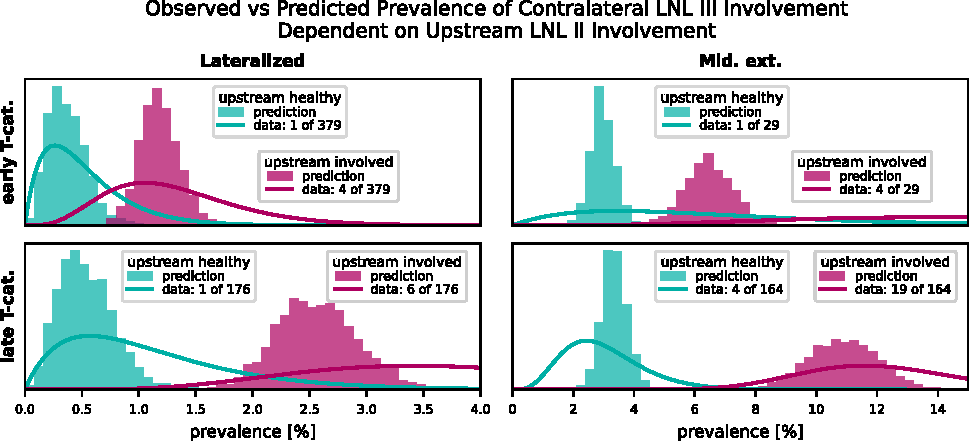
\includegraphics{manuscript_files/mediabag/figures/fig_model_prevalences_upstream.pdf}

}

\caption{\label{fig-model-prevalences-upstream}The influence of the
upstream LNL II's involvement on the prevalence of contralateral level
III for the four combinations of tumor lateralization (lateralized or
extending over midline) and T-ctageory (early or advanced). Our model
predictions (histograms) are plotted against the observations in the
data (beta posteriors).}

\end{figure}%

Figure~\ref{fig-model-prevalences-upstream} illustrates how rarely the
contralateral LNL III harbors metastases when its upstream level II is
healthy. Also, the model can capture this correlation rather well, with
the exception of early T-category tumors that extend over the
mid-sagittal line. As in figure~\ref{fig-model-prevalences-overall} and
figure~\ref{fig-model-prevalences-with-ipsi}, these cases are relatively
rare resulting in a broad distribution over the true prevalence.

\subsubsection{Prevalence of Midline
Extension}\label{prevalence-of-midline-extension}

\begin{figure}

\centering{

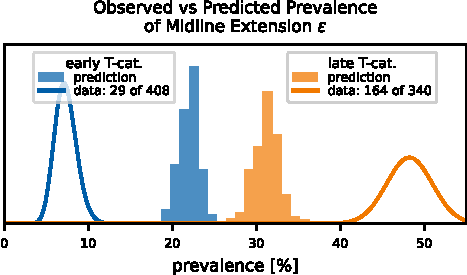
\includegraphics[width=0.5\textwidth,height=\textheight]{manuscript_files/mediabag/figures/fig_model_prevalences_midext.pdf}

}

\caption{\label{fig-model-prevalences-midext}Comparing the predicted
(histograms) and observed (lines depicting beta posteriors) prevalence
of midline extension for early (blue) and late (orange) T-category.
While the prevalence is predicted correctly when marginalizing over
T-category, the model cannot capture the degree of separation observed
in the data. Since the tumor's midline extension is virtually always
part of the diagnosis and hence \emph{given} when predicting a patient's
risk, we do not consider this discrepancy a major issue.}

\end{figure}%

Lastly, in figure~\ref{fig-model-prevalences-midext}, we plot the
prevalence of midline extension in the data versus our model's
prediction. It is obvious the model cannot match the large spread
between early and advanced T-category seen in the data. This is because
to achieve that, it would need to increase the advanced T-category
patient's prior distribution over diagnosis times and at the same time
reduce the probability of the tumor to cross the midline during a
time-step. But since the time-priors parameter is also coupled with the
spread probabilities among the LNLs, the model does not have that
freedom.

However, we do not consider this discrepancy a major limitation of the
model: We will not realistically be interested in the probability of
midline extension, as it is always possible to assess it with high
certainty. That is also the reason why we initially modelled the midline
extension \emph{not} as a random variable, but as a global risk factor
that would have been turned on or off from the onset of a patient's
disease evolution. This, however, lead to overly high risks for
contralateral involvement in advanced T-category patients with midline
extension, because then the model assumes an increased spread to the
contralateral side from the onset of the disease. Which is probably not
true in a majority of those cases. Thus, treating it as a random
variable that only becomes true during a patient's disease evolution
resulted in a better description of the data.

Formally, the wrong prediction of midline extension prevalence makes
little difference, since it is always given: Instead of
\(P\left( \mathbf{X}^\text{i}, \mathbf{X}^\text{c}, \epsilon \mid \mathbf{Z}^\text{i}, \mathbf{Z}^\text{c} \right)\),
we typically compute
\(P\left( \mathbf{X}^\text{i}, \mathbf{X}^\text{c} \mid \mathbf{Z}^\text{i}, \mathbf{Z}^\text{c}, \epsilon \right)\),
which does not suffer from the wrong probability of midline extension,
as the distribution over hidden states is renormalized:

\[
P \left( \mathbf{X}^\text{i}, \mathbf{X}^\text{c} \mid \mathbf{Z}^\text{i}, \mathbf{Z}^\text{c}, \epsilon \right) = \frac{P \left( \mathbf{Z}^\text{i}, \mathbf{Z}^\text{c} \mid \mathbf{X}^\text{i}, \mathbf{X}^\text{c}, \epsilon \right) P \left( \mathbf{X}^\text{i}, \mathbf{X}^\text{c}, \epsilon \right)}{P \left( \mathbf{Z}^\text{i}, \mathbf{Z}^\text{c}, \epsilon \right)}
\]

Note that a distribution over \(\epsilon\) appears both in the
enumerator and the denominator, which largely cancel each other, leaving
only the midline extension's effect on the distribution over hidden
states in the prediction.

Also, the discrepancy in midline extension prevalence between early and
advanced T-category is particularly pronounced in oropharyngeal SCC
patients. For example, in oral cavity SCC, the midline extension only
increases from 15.4\% (20 out of 130) to 33.3\% (13 out of 39).

\section{Results: Prediction of Risk for Occult
Disease}\label{results-prediction-of-risk-for-occult-disease}

For a clinical application of the model we are interested in the risk of
occult metastases rather than the observed patterns of lymph node
involvement. We want to estimate the risk for occult disease in
clinically negative LNLs, given the patient's individual diagnosis. In
terms of our model, the diagnosis consists of the T-category, the
lateralization of the tumor (if it extend over the mid-sagittal plane),
and which LNLs are clinically involved based on imaging and possibly
fine needle aspiration (FNA). For the results shown in this section, we
assume that involvement of a LNL is clinically diagnosed through imaging
with a sensitivity of 81\% and a specificity of 76\%
\citep{de_bondt_detection_2007}. For FNA we assume a specificity of 98\%
and a sensitivity of 80\%. This amounts to the assumption that lymph
node involvement confirmed by FNA is almost certainly true involvement,
i.e.~there are almost no false positive diagnoses.

\begin{figure}

\centering{

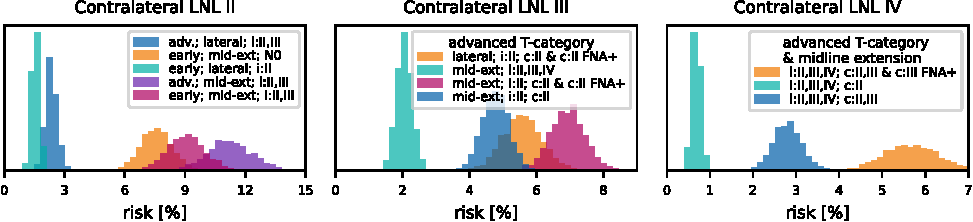
\includegraphics{manuscript_files/mediabag/figures/fig_model_risks.pdf}

}

\caption{\label{fig-model-risks}Histograms over the predicted risk of
occult contralateral LNL II (left), III (middle), and IV (right)
invovlement, shown for some combinations of T-category, tumor
lateralization, and clinical LNL diagnoses. All LNLs not explicitly
mentioned in the legend, including the LNL for which the risk of occult
disease was computed, where assumed to be clinically negative, based on
CT imaging (specificity 76\%, sensitivity 81\%).}

\end{figure}%

\subsection{Contralateral LNL II}\label{contralateral-lnl-ii}

Figure~\ref{fig-model-risks} (left panel) shows the predicted risk of
occult disease in contralateral LNL II. The most important variable
impacting the prediction for contralateral level II involvement in our
model is the tumor's lateralization. A patient with a clearly
lateralized early T-category tumor and a clinically N0 neck is predicted
to have a 1-2\% risk for occult disease in contralateral LNL II. For a
patient with a clearly lateralized early T-category tumor but
\emph{with} mid-sagittal extension, the risk increases to almost 7\%.

Also advanced T-category increases the risk of occult disease but plays
a lesser role: Considering the scenario of a tumor that crosses the
midline and an ipsilateral neck where at least LNL III is clinically
involved, the risk for occult contralateral LNL II disease is around
8.5\%. For the same scenario and an advanced T-category tumor, the risk
increases to 11\%.

Lastly, the predicted risk is also correlated via the time-steps to the
degree of ipsilateral involvement. Changing the aforementioned scenario
(advanced T-category, midline extension, ipsilateral LNL III clinically
involved) to one where the patient presents with a clinically N0 neck,
the risk for occult disease in the contralateral LNL II falls from 11\%
to 9.5\%.

Taken together, T-category and ipsilateral involvement may still
considerably impact the risk prediction for contralateral involvement:
In figure~\ref{fig-model-risks} the scenarios underlying the orange
(6.5\% ) and the red (11\% ) histograms differ in T-category (early vs
advanced) and clinical diagnosis (N0 vs ipsilateral at least LNL III
involved).

\subsection{Contralalteral LNL III}\label{contralalteral-lnl-iii}

As shown in the center subplot of figure~\ref{fig-model-risks}, the risk
for occult disease in the contralateral LNL III may only cross a 5\%
threshold if the upstream level II is clinically involved, too. If the
clinical diagnosis of the contralateral upstream level II is
pathologically confirmed by FNA the risk increases by another percentage
point. When the tumor additionally crosses the mid-sagittal line, the
risk may reach around 7\%.

\subsection{Contralateral LNL IV}\label{contralateral-lnl-iv}

Our model's prediction for the contralateral LNL IV show that even in
the most extreme case, with an advanced T-category tumor extending over
the mid-sagittal line as well as metastases in every ipsilateral LNL and
every contralateral upstream level, the risk stays just below 3\%. We
only observe a risk of 5-6\% when the involvement of the upstream level
III is pathologically confirmed after taking a biopsy using FNA. This is
because the model's prior probability for contralateral LNL IV
involvement is so low that even given a clinical diagnosis in that
level, a false positive in LNL III is a more likely explanation. This
possibility, however, drops virtually to zero when tumor cells are
pathologically confirmed in level III.

\section{Discussion}\label{sec-discussion}

\subsection{Summary}\label{summary}

In this work we present a formalism to model the ipsi- and contralateral
lymphatic involvement of oropharyngeal SCC patients. An ipsilateral
model has been previously developed and published
\citep{ludwig_hidden_2021, ludwig_modelling_2023}. Based on this, we
introduce an extension that leaves the ipsilateral model untouched, but
extends it to the contralateral side in an intuitive and comprehensible
manner.

The model's performance w.r.t. its ability to describe the data on
contralateral nodal involvement was evaluated based on a dataset of 833
patients from four institutions. To the best of our knowledge, this is
the first time lymphatic tumor progression has been modelled in such
detail and to such an extent. While there was work on regional tumor
spread, these models were conceptually different, more limited in the
LNLs for which they make predictions, and not trained with real patient
data \citep{benson_markov_2006, jung_development_2017}.

The model takes the clincal diagnosis of the lymph node levels, the
primary tumor's T-category, as well as lateralization into account when
predicting the personalized risk for occult disease in any LNL of
interest. Owing to the relatively few parameters, the model is highly
interpretable and every parameter can be intuitively explained, while
still offering good accuracy in its predictions.

\subsection{Implications for Contralateral Elective Nodal
Treatment}\label{implications-for-contralateral-elective-nodal-treatment}

The predictions of this model are being used to inform a clinical trial
on volume deescalation at the University Hospital Zurich {[}citation
needed{]}. When accepting a 5\% risk of occult disease in any given LNL,
the model suggests the following contralateral elective irradiation
(assuming the respective LNL appears clinically healthy):

\begin{itemize}
\tightlist
\item
  LNL II when the tumor extends over the mid-sagittal line
\item
  LNL III when LNL II is clinically involved, may need confirmation via
  FNA
\item
  LNL IV only when upstream level III pathologically confirmed
\end{itemize}

\section{Acknowledgement}\label{acknowledgement}

This work was supported by:

\begin{itemize}
\tightlist
\item
  the Clinical Research Priority Program ``Artificial Intelligence in
  Oncological Imaging'' of the University of Zurich
\item
  the Swiss Cancer Research Foundation under grant number KFS
  5645-08-2022
\end{itemize}

\section{Contralateral Prevalence of
Involvement}\label{contralateral-prevalence-of-involvement}

\textsubscript{Source:
\href{https://rmnldwg.github.io/bilateral-paper/manuscript-preview.html}{Article
Notebook}}

\begin{longtable}[]{@{}llllllllllll@{}}

\caption{\label{tbl-data-strat}Contralateral involvement depending on
whether the primary tumor extends over the mid-sagittal line, the
T-category, and whether the ipsilateral LNL III was involved or
healthy.}

\tabularnewline

\caption{}\label{T_a95ce}\tabularnewline
\toprule\noalign{}
T-cat. & ipsi & Mid. ext. & \multicolumn{2}{l}{%
I} & \multicolumn{2}{l}{%
II} & \multicolumn{2}{l}{%
III} & \multicolumn{2}{l}{%
IV} & total \\
& & & n & \% & n & \% & n & \% & n & \% & n \\
\midrule\noalign{}
\endfirsthead
\toprule\noalign{}
T-cat. & ipsi & Mid. ext. & \multicolumn{2}{l}{%
I} & \multicolumn{2}{l}{%
II} & \multicolumn{2}{l}{%
III} & \multicolumn{2}{l}{%
IV} & total \\
& & & n & \% & n & \% & n & \% & n & \% & n \\
\midrule\noalign{}
\endhead
\bottomrule\noalign{}
\endlastfoot
early & 0 & False & 0 & 0.00 & 1 & 1.16 & 0 & 0.00 & 0 & 0.00 & 86 \\
early & 0 & True & 0 & 0.00 & 1 & 10.00 & 1 & 10.00 & 0 & 0.00 & 10 \\
early & 1 & False & 1 & 0.53 & 11 & 5.82 & 2 & 1.06 & 1 & 0.53 & 189 \\
early & 1 & True & 1 & 11.11 & 2 & 22.22 & 0 & 0.00 & 0 & 0.00 & 9 \\
early & ≥ 2 & False & 1 & 0.96 & 15 & 14.42 & 3 & 2.88 & 3 & 2.88 &
104 \\
early & ≥ 2 & True & 0 & 0.00 & 3 & 30.00 & 4 & 40.00 & 1 & 10.00 &
10 \\
advanced & 0 & False & 0 & 0.00 & 2 & 5.88 & 0 & 0.00 & 0 & 0.00 & 34 \\
advanced & 0 & True & 0 & 0.00 & 3 & 12.50 & 0 & 0.00 & 0 & 0.00 & 24 \\
advanced & 1 & False & 0 & 0.00 & 3 & 4.55 & 0 & 0.00 & 0 & 0.00 & 66 \\
advanced & 1 & True & 1 & 1.64 & 18 & 29.51 & 5 & 8.20 & 1 & 1.64 &
61 \\
advanced & ≥ 2 & False & 4 & 5.26 & 16 & 21.05 & 7 & 9.21 & 4 & 5.26 &
76 \\
advanced & ≥ 2 & True & 3 & 3.80 & 46 & 58.23 & 18 & 22.78 & 8 & 10.13 &
79 \\

\end{longtable}

\textsubscript{Source:
\href{https://rmnldwg.github.io/bilateral-paper/manuscript-preview.html}{Article
Notebook}}


  \bibliography{references.bib}



\end{document}
